% GRUNDEINSTELLUNGEN -------------------------------------------

\documentclass[a4paper]{article}
\usepackage[ngerman]{babel}
\usepackage[utf8]{inputenc}


% EINGEBUNDENE PAKETE ------------------------------------------

\usepackage{pdfpages} % andere PDFs einbinden
\usepackage{verbatim} % program listings
\usepackage{latexsym} % Symbole zB Box
\usepackage{amssymb} % z.B. mathbb{}
\usepackage{amsmath} 
\usepackage{amsthm} % Für Lemmata, Sätze(Theoreme), Beweise (siehe unten)
\usepackage{tikz}	% Für Diagramme aus dem Programm Dia
\usepackage{makeidx} % fuer Stichwortverzeichnis
\usepackage{csquotes}
\usepackage{color}

% Verweise anklickbar machen
\usepackage{hyperref} % 1. 
\usepackage[figure]{hypcap} % 2. 


% EIGENE BEFEHLE -----------------------------------------------
% Bildbreite: Originalgröße oder falls größer als Seitenbreite/Spalte ==> skalieren
\makeatletter
\def\ScaleIfNeeded{%
\ifdim\Gin@nat@width>\linewidth
\linewidth
\else
\Gin@nat@width
\fi
}
\makeatother

% Neuer Befehl der Bilder standartisiert einbindet:
% includegraphicsdeluxe benötigt \ScaleIfNeeded und \ldate
% 1. innerhalb der figure-Umgebung mit dem Versuch, das Bild mittels [!htb] an genau dieser Position einzufügen
% 2. mit der Original- oder einer skalierten (mittels ScaleIfNeeded s.o.) Größe
% 3. mit einer Beschriftung (\caption{})
% 4. mit einem Label (\label{})
\newcommand{\includegraphicsdeluxe}[4]{
	\begin{figure}[!htb] 
	\centering
	\includegraphics[width=1\ScaleIfNeeded]{pics/\ldate_#1}
	\caption[#2]{#3}
	\label{#4}
	\end{figure}
}


% AND und OR Symbole
\newcommand{\und}{\wedge}
\newcommand{\oder}{\vee}

% Grundmengen
\newcommand{\N}{\mathbb{N}}
\newcommand{\Z}{\mathbb{Z}}
\newcommand{\Q}{\mathbb{Q}}
\newcommand{\R}{\mathbb{R}}
\newcommand{\C}{\mathbb{C}}

% größenangepasste Betragsstriche, Klammern, ...
\newcommand{\abs}[1]{\ensuremath{ \left\vert #1 \right\vert }}
\newcommand{\rbr}[1]{\ensuremath{ \left( #1 \right) }} % round brackets ()
\newcommand{\cbr}[1]{\ensuremath{ \left\lbrace #1 \right\rbrace }} % curly brackets {}
\newcommand{\sbr}[1]{\ensuremath{ \left[ #1 \right] }} % square brackets []

% Vektoren mit Klammern und so 
\newcommand{\vektor}[1]{\ensuremath{ \rbr{ \begin{array}{c} #1 \end{array} } }} 

% Sonderzeichen
\newcommand{\grad}{$^\circ$}
\newcommand{\gradi}{^\circ}

% Deltas
\newcommand{\Dt}{\Delta t}
\newcommand{\Dx}{\Delta x}
\newcommand{\Dy}{\Delta y}
\newcommand{\DA}{\Delta \alpha}
\newcommand{\DPH}{\Delta \varphi}
\newcommand{\Ds}{\Delta s}

\newcommand{\dt}{\delta t}
\newcommand{\dx}{\delta x}
\newcommand{\dy}{\delta y}
\newcommand{\df}{\delta f}
\newcommand{\dz}{\delta z}


% lokale Platzhalter
\newcommand{\locpl}{}

% Datum der einzelnen Lektionen definieren
\newcommand{\ldate}{2015-10-01}	% define lessiondate

% Anmerkung Professor
\newcommand{\profnote}[1]{\marginpar{\tiny{\textquote{#1}}}}

% Dokumenteneigenschaften
\newcommand{\pTitle}{Differentialrechnung in $\R^n$ und Differentialgleichungen}
\newcommand{\pShortName}{M. Zell}
\newcommand{\pSemester}{WS 2015/16}
\newcommand{\pProfessor}{Prof. Dr. Josef Hörwick}

% EINRÜCKUNG ---------------------------------------------------
\setlength{\parindent}{0pt} % Erste Zeile in Absätzen nicht einrücken.

% KOPF- UND FUSSZEILE ------------------------------------------
\usepackage{fancyhdr}
\pagestyle{fancy}
\fancyhf{}
 
%Kopfzeile mittig mit Kaptilname
\fancyhead[L]{\textsf{\nouppercase{\leftmark}}}
\fancyhead[R]{\textsf{\thepage}}
%Linie oben
\renewcommand{\headrulewidth}{0.5pt}
%Fußzeile 
\fancyfoot[L]{\tiny{\pTitle}}
\fancyfoot[R]{\tiny{\pShortName, \pSemester, \ldate}}
%Linie unten
\renewcommand{\footrulewidth}{0.5pt}
 
% START DES EIGENTLICHEN DOKUMENTS -----------------------------
\author{\pShortName}
\title{Mitschrift\\\pTitle, \pSemester\\\pProfessor}

% Stichwortverzeichnis erstellen
\makeindex

\begin{document}
\maketitle
\newpage
\tableofcontents
\newpage
\listoffigures

% Sätze usw. aus asmthm
\newtheorem{satz}{Satz}[section] 
\newtheorem{defi}{Definition}[section] 
\newtheorem{lem}{Lemma}[section] 
\newtheorem{beh}{Behauptung}[section] 

% einzelne Kapitel
\renewcommand{\ldate}{2015-10-01}

\section{Hinweise}
Diese Mitschrift basiert auf der Vorlesung \textquote{\pTitle} von \pProfessor \ im \pSemester. Du kannst sie gerne benutzen, kopieren und an andere weitergeben. Auch in der Prüfung - soweit zugelassen \footnote{\url{http://www.cs.hm.edu/meinstudium/studierenden_services/fi_pruefungskatalog.de.html}} - kannst du sie gerne als Hilfsmittel verwenden, wenn das meine Nutzung als Prüfungshilfsmittel nicht in irgendeiner Weise beeinträchtigt.\\

Natürlich besteht kein Anspruch auf Aktualität, Richtigkeit, Fortsetzung meines Angebots oder dergleichen. Sollten dir Fehler auffallen oder solltest du Verbesserungsvorschläge haben, würde ich mich über eine E-Mail (zell@hm.edu) freuen. Wenn du mir als kleines Dankeschön z.B. ein Club-Mate\footnote{\url{http://www.clubmate.de/ueber-club-mate.html}} ausgeben möchtest, findest du mich meistens hier: \url{http://fi.cs.hm.edu/fi/rest/public/timetable/group/if3b}. Wenn nicht, ist es auch ok ;-)\\

Nach der Prüfung werde ich den \LaTeX-Quelltext veröffentlichen, damit die Mitschrift weitergeführt, korrigiert und ergänzt werden kann.\\

Viele Grüße\\
\pShortName
% Vorlesung vom 01.10.2015
\renewcommand{\ldate}{2015-10-01}	% define lessiondate

\section{Abbildungen des Typs $\R^n \rightarrow \R$}
$f: 
\begin{cases}
 \R^2 \rightarrow \R\\
 (x,y)\rightarrow f(x,y)
\end{cases}
$
Zwei Variablen. \profnote{Gebirge über der x,y-Ebene.} 

\includegraphicsdeluxe{schnittfunktionen.jpg}{Schnittfunktionen im $ \R^n $}{Schnittfunktion parallel zur yz-Ebene (rot); Schnittfunktion parallel zur xz-Ebene (blau).}{fig:schnittfunktionen} 

Die Ableitungen der Schnittfunktionen heißen partielle Ableitungen. $\frac{\delta f}{\delta x} (x,y)$ ist die Ableitung der blauen Funktion (nur x ist Variable). $\frac{\delta f}{\delta y} (x,y)$ ist die Ableitung der roten Funktion (nur y ist Variable).

\subsection{Beispiele}

\paragraph{a)} $f(x,y)= 2x^3y^2 + x+2y $\\
$\frac{\delta f}{\delta x} = 2y^2 3x^2 + 1 $\\
$\frac{\delta f}{\delta y} = 2x^3 2y + 2 $

\paragraph{b)} $f(x,y) = \sin(x y^2)$\\
$\frac{\delta f}{\delta x} = \cos(x y^2) y^2$\\
$\frac{\delta f}{\delta y} = \cos(x y^2) x 2y$

\subsection{Verallgemeinerung}
$f: 
\begin{cases}
 \R^n \rightarrow \R\\
 (x_1, ..., x_n) \rightarrow f(x_1, ..., x_n)\\
\end{cases}
$\\

$\frac{\delta f}{\delta x_1} (x_1, ..., x_n)$ nur $x_1$ ist Variable.\\
$\vdots$\\
$\frac{\delta f}{\delta x_n} (x_1, ..., x_n)$ nur $x_n$ ist Variable.\\
Zum Beispiel: $\frac{\delta f}{\delta x_1}$\\
%2 \includegraphicsdeluxe{.jpg}{}{}{fig:}

\subsection{Beispiele}
\paragraph{a)} $f(x,y,z) = x^5y^2z^3 + xy + z^2$\\
$\frac{\delta f}{\delta x} = 5x^4 y^2 z^3 + y$\\
$\frac{\delta f}{\delta y} = 2y x^5 z^3 + x$\\
$\frac{\delta f}{\delta z} = 3z^2 x^5 y^2 + 2z$\\

\paragraph{b)} $ f(x,y,z) = e^{2x} e^y + z^2 \sin(x) $\\
$\frac{\delta f}{\delta x} = e^{2x} 2 e^y + \cos(x) z^2 $\\
$\frac{\delta f}{\delta y} = e^{2x} e^y $\\
$\frac{\delta f}{\delta z} = 2z  \sin(x) $\\

\paragraph{c)} $ f(x,y,z) = e^x \sin(xy) + yz  e^z $\\
$\frac{\delta f}{\delta x} = e^x \sin(xy) + e^x \cos(xy) y $\\
$\frac{\delta f}{\delta y} = e^x \cos(xy) x + z e^z $\\
$\frac{\delta f}{\delta z} = y e^z + yz e^z$\\


\subsection{Linearisierung von Funktionen $\R^2 \rightarrow \R$} 
\profnote{Heißt nichts anderes als ich ersetze die Funktion durch die Tangente. Dadurch kann man eine schwierige Funktion durch eine einfachere ersetzen.}

Ersetze das Funktionsgebirge im Punkt (x,y,z) durch die Tangentialebene $\varepsilon$. Dieses $\varepsilon$ wird aufgespannt durch die beiden Tangenten an die beiden Schnittfunktionen (siehe Abb. \ref{fig:tangentialebene1}). 

\includegraphicsdeluxe{tangentialebene1.png}{Tangentialebene anstelle eines Funktiongebirges}{Die orangenen Tangenten an die blaue und die rote Schnittfunktion spannen eine Tangentialebene auf. Diese entspricht dem $ \varepsilon $. Es gilt: blaue Schnittfunktion: $ \frac{\delta f}{\delta x} (x,y) dx $, rote Schnittfunktion: $ \frac{\delta f}{\delta y} (x,y) dy $ und dz = $\frac{\delta f}{\delta x} (x,y) dx + \frac{\delta f}{\delta y} (x,y) dy $ }{fig:tangentialebene1}

\subsection{Linearisierungsformel}
$ f(x+dx, y+dy) \approx f(x,y) + \frac{\delta f}{\delta x} (x,y) dx + \frac{\delta f}{\delta y} (x,y) dy $

\profnote{Mit dieser Formel können wir die Funktion im Punkt (x,y) durch die Tangentialebene ersetzen.}

\subsection{Beispiel} Linearisiere $f(x,y)=x^2 y^3$ bei $x=2,y=1$\\
$ \frac{\delta f}{\delta x} = 2x y^3$\\
$ \frac{\delta f}{\delta y} = 3y^2 x^2$\\
$ f(x+dx, y+dy) \approx x^2 y^3 + 2xy^3 \cdot dx + 3y^2x^2 \cdot dy $\\
$ f(2,1) = 4 $\\
$ \frac{\delta f}{\delta x} (2,1) = 2 \cdot 2 \cdot 1 = 4$\\
$ \frac{\delta f}{\delta y} (2,1) = 3 \cdot 4 = 12$\\
$ \Rightarrow f(2+dx,1+dy) \approx 4+4 \cdot dx+12 \cdot dy$

\textbf{Test} mit $dx=0.1, dy=-0.1$\\
$ f(2.1, 0.9) = 2.1^2 0.9^3 = \textbf{3.214...}$\\
$ f(2+0.1, 1-0.1) \approx 4+4 \cdot 0.1-12\cdot 0.1 = 4+0.4-1.2=\textbf{3.2} \checkmark $

\subsection{Verallgemeinerung} 
$ f(x_1+dx_1, x_2+dx_2,..., x_n+dx_n) \approx f(x_1,...,x_n) + \frac{\delta f}{\delta x_1} \cdot dx_1 + ... + \frac{\delta f}{\delta x_n} \cdot dx_n$
% Vorlesung vom 02.10.2015
\renewcommand{\ldate}{2015-10-02}	% define lessiondate

\subsection{Beispiel} Linearisiere
$ f(x,y,z) = x  \sin y + y  \cos z$ bei (0.5, 1, 0.9)\\
$ f(0.5, 1, 0.9) = 0.5 \sin 1 + 1  \cos 0.9 = 1.042 $ \profnote{In der Mathematik gilt: Wenn man sich nicht sicher ist, immer den Winkel im Bogenmaß eingeben.}\\
$ \frac{\delta f}{\delta x} = \sin(y) \widehat{=} \sin(1) = 0.841 $ \\
$ \frac{\delta f}{\delta y} = x \cos(y) + \cos(z) \widehat{=} 0.5 \cos 1 + \cos 0.9 = 0.892 $ \\
$ \frac{\delta f}{\delta z} = -y \sin z \widehat{=} -1 \sin 0.9 = -0.783$ \\
\textbf{Test:} $ f(0.5+dx,1+dy,0.9+dz) \approx 1.042+0.841 dx + 0.892 dy - 0.783 dz$ z.B.: $ f(0.5+0.1,1+0.1,0.9-0.1) \approx ... = 1.293$. Der exakte Wert: $ f(0.6, 1.1, 0.8) = 1.301...$

\subsection{Anwendung der Linearisierung - Die Fehlerrechnung}
Gegeben ist $ f(x_1, ..., x_n)$. Die Größen $ x_1, ..., x_n $ werden gemessen, wobei $x_1 = \overline{x_1} + w_1$ (wahrer Wert, Messwert und Fehler), ..., $x_n = \overline{x_n} + w_n$.\\
Wahres Ergebnis: $ e = f(x_1, ..., x_n) $\\
Fehlerhaftes Ergebnis: $ \overline{e} = f(\overline{x_1}, ..., \overline{x_n}) $\\ 
$ \Rightarrow e = f(\overline{x_1}+w_1, ..., \overline{x_n}+w_n) $. Wir linearisieren an der Messstelle: $ e = f(\overline{x_1}, ..., \overline{x_n}) + \frac{\delta f}{\delta x_1} (\overline{x_1},...,\overline{x_n}) w_1 + ... + (\overline{x_1},...,\overline{x_n}) w_n $. Die Fehler $w_1, ..., w_n$ kennt man nicht. Gegeben sind die maximalen Fehler der Messwerte: $x_i = \overline{x_i} \pm \Delta x_i$. Der maximale Fehler des Ergebnisses ist: 
\[
\abs{\frac{\delta f}{\delta x_1} (\overline{x_1},...,\overline{x_n}) \Delta x_1 } + ... + \abs{\frac{\delta f}{\delta x_n} (\overline{x_1},...,\overline{x_n}) \Delta x_n}
\]

\subsection{Beispiel}
$ f(x_1,x_2,x_3,x_4) = x_1^2  \sin(x_2) + x_3 x_4  \cos x_2 $\\
$x_1 = 10m \pm 5cm$\\
$x_2=40^\circ \pm 1^\circ \widehat{=} 0.01745 rad$\\
$x_3=12m \pm 6cm$\\
$x_4=7m\pm 4cm$\\
$f(10m,40^\circ,12m,7m) = 128.6m^2$\profnote{Je nach Rundungsgenauigkeit können die Ergebnisse leicht abweichen.}\\
$\frac{\delta f}{\delta x_1} = 2x_1 \sin x_2 \widehat{=} 2 \cdot 10 \sin 40^\circ = 12.86$\\
$\frac{\delta f}{\delta x_2} = x_1^2 \cos x_2 - x_3 x_4 \sin x_2 \widehat{=} 22.61$\\
$\frac{\delta f}{\delta x_3} = x_4 \cos x_2 \widehat{=} 5.36$\\
$\frac{\delta f}{\delta x_4} = x_3 \cos x_2 \widehat{=} 9.19$\\
maximaler Fehler $= |12.85 \cdot 0.05|+|22.61 \cdot 0.01745|+|5.36 \cdot 0.06|+|9.19 \cdot 0.04| = 0.64 + 0.39 + 0.32 + 0.37 = (\textrm{von } \Delta x_1 \Delta x_2 \Delta x_3 \textrm{ und }\Delta x_4) = 1.73 $

\subsection{Die Richtungsableitung}
Wir betrachten $ f: \R^n \rightarrow \R$. Wir wollen nun die Richtungsableitung des Vektors $ v \in \R^n, |v| = 1 $ aufstellen (Abb. \ref{fig:richtungsableitung1}). 
Dazu betrachten wir die Funktion entlang der Geraden g (Abb. \ref{fig:richtungsableitung2}) und erhalten: $ f_v(x_1,...,x_n) = \lim\limits_{h\rightarrow 0} \frac{f((x_1,...,x_n)+h(v_1,...,v_n)) - f(x_1,...,x_n)}{h} $

\includegraphicsdeluxe{richtungsableitung1.jpg}{Richtungsableitung im Raum}{Der rote Vektor v liegt auf der Geraden g und im Raum $ \R^n $}{fig:richtungsableitung1}

\includegraphicsdeluxe{richtungsableitung2.jpg}{Richtungsableitung entlang der Geraden g}{Wir betrachten die Funktion entlang g.}{fig:richtungsableitung2}

\subsection{Beispiel} 
$ f: \R^3 \rightarrow \R, (x_1,x_2,x_3) \rightarrow x_1 x_2 + 2x_3\\
\tilde{v}=(1,2,2), |\tilde{v}|=\sqrt{1^2+2^2+2^2}=3, v=\frac{1}{3}(1,2,2)=(\frac{1}{3},\frac{2}{3},\frac{2}{3})\\
f_v(x_1,x_2,x_3)=\lim\limits_{h\rightarrow 0} \frac{f((x_1,x_2,x_3)+h(v_1,v_2,v_3)) - f(x_1,x_2,x_3)}{h}= 
\lim\limits_{h\rightarrow 0} \frac{f((x_1+\frac{1}{3} h,x_2+\frac{2}{3} h,x_3+\frac{2}{3} h)) - f(x_1,x_2,x_3)}{h}= 
\lim\limits_{h\rightarrow 0} \frac{f((x_1+\frac{1}{3} h,x_2+\frac{2}{3} h,x_3+\frac{2}{3} h)) - x_1 x_2 - 2x_3}{h}= 
\lim\limits_{h\rightarrow 0} \frac{x_1 x_2 + x_1 \frac{2}{3} h + \frac{1}{3} h x_2 + \frac{2}{9} h^2 + 2x_3 + \frac{4}{3} h - x_1 x_2 - 2x_3}{h}=
\lim\limits_{h\rightarrow 0} \frac{2}{3} x_1 + \frac{1}{3} x_2 + \frac{2}{9} h + \frac{4}{3} = \frac{2}{3} x_1 + \frac{1}{3} x_2 + \frac{4}{3} \Rightarrow 
f_v(x_1,x_2,x_3) = \frac{2}{3} x_1 + \frac{1}{3} x_2 + \frac{4}{3}  $


% Vorlesung vom 08.10.2015
\renewcommand{\ldate}{2015-10-08}

\subsection{Definition}
Wiederholung Richtungsableitung: $ f_v(x)=\lim\limits_{h\rightarrow 0} \frac{f(x+h\cdot v) - f(x)}{h}$
\begin{defi}
$ f: \R^n \rightarrow R $\\
Der Vektor ($ \frac{\delta f}{\delta x_1}, \frac{\delta f}{\delta x_2}, ..., \frac{\delta f}{\delta x_n} $) heißt der Gradient von f bei x.
\end{defi}

\begin{satz}
$ f: \R^n \rightarrow \R $\\
$ v = (v_1, ..., v_n) \textrm{mit} |v|=1 $
Dann gilt: $ f_v(x_1, ..., x_n) = (v_1, ..., v_n) \cdot \frac{\delta f}{\delta x_1}, \frac{\delta f}{\delta x_2}, ..., \frac{\delta f}{\delta x_n} $\\
$ f_v(x) = v \cdot \textrm{Gradient von f} (\widehat{=} \textrm{ Skalarprodukt: } (x_1,x_2)\cdot (y_1,y_2)=x_1y_1+x_2+y_2) $ 
\end{satz}

% \profnote{Jetzt machen wir einen Beweis. Wenn man den schlampig macht, geht's recht schnell. Wir machens schlampig.}

\begin{proof}
$ f(x_1+dx_1, ..., x_n+dx_n) \approx f(x_1, ..., x_n) + \frac{\delta f}{\delta x_1} \cdot dx_1 + ... + \frac{\delta f}{\delta x_n} \cdot dx_n  $\\
$ f(x_1+h v_1,x_2+h v_2, ..., x_n+h v_n) $
$ \approx f(x_1, ..., x_n) + \frac{\delta f}{\delta x_1} \cdot h\cdot v_1 + ... + \frac{\delta f}{\delta x_n} \cdot h\cdot v_n $\\
Einsetzen der Grenzwertbildung:\\
$ \lim\limits_{h\rightarrow 0} = \frac{f(x_1+hv_1,...,x_n+hv_n) - f(x_1, ..., x_n)}{h} $
$ = \lim\limits_{h\rightarrow 0} \frac{f(x_1,...x_n)+\frac{\delta f}{\delta x_1}hv_1 + ... + \frac{\delta f}{\delta x_n}hv_n - f(x_1, ..., x_n)}{h} $ 
$ = \lim\limits_{h\rightarrow 0} = \frac{\delta f}{\delta x_1} v_1 + ... + \frac{\delta f}{\delta x_n} v_n = \textrm{Gradient von f} \cdot v $
\end{proof}

\subsection{Beispiel von oben}
$ f(x_1,x_2,x_3) = x_1x_2 + 2x_3, v=(\frac{1}{3}, \frac{2}{3}, \frac{2}{3}) $\\
$ f_v(x_1,x_2,x_3)=(v_1,v_2,v_3)\cdot (\frac{\delta f}{\delta x_1}, \frac{\delta f}{\delta x_2}, \frac{\delta f}{\delta x_3}) $
$ = (\frac{1}{3}, \frac{2}{3}, \frac{2}{3})\cdot (x_2, x_1, 2) = \frac{1}{3} x_2 + \frac{2}{3} x_1 + \frac{4}{3} $

\subsection{Hausaufgabe}
% \profnote{Das können Sie zu Hause rechnen. }
$ f(x_1, x_2, x_3, x_4) = x_1^2 x_2 x_3 + x_3^2 x_4$\\
Richtung $ \tilde{v} = (1,-1,-1,1) $ \\
Richtungsableitung in: $ (1,0,2,-1) $

\subsection{Problem} $ f:\R^n \rightarrow \R $
Folgende Fragen stellen wir uns: 
\begin{itemize}

\includegraphicsdeluxe{steilsteRichtungsableitung.jpg}{Steilste Richtungsableitung}{In welcher Richtung geht es am steilsten bergauf?}{fig:steilste_richtungsableitung1}

\item In welcher Richtung v ist die Richtungsableitung am größten?
\item In welcher Richtung wächst die Funktion am schnellsten?
\item In welcher Richtung geht es am steilsten Bergauf? (Abb. \ref{fig:steilste_richtungsableitung1})
\end{itemize}

\includegraphicsdeluxe{gradientf.jpg}{Gradient von f}{Gradient von f}{fig:gradientf1} 

$ \cos = \frac{v gradf}{|v| \cdot |gradf|} = \frac{f_v}{|gradf|} \Rightarrow f_v=\cos \delta \cdot |gradf| $ (Abb. \ref{fig:gradientf1}). $f_v$ ist maximal bei $\cos \delta = 1$, d.h. bei $\delta=0^\circ$. Die Richtungsableitung ist maximal in Richtung gradf. Die maximale Richtungsableitung ist $|gradf|$. 

\subsection{Beispiel}
$ f(x_1,x_2,x_3) = 3x_1x_2 + 2x_3^2 $\\
Punkt: (1,2,-2)\\
In welcher Richtung wächst f am stärksten? \\
$ gradf = (3x_2, 3x_1, 4x_3) $\\
$ gradf(1,2,-2) = \underline{(6,3,-8)} $ (gesuchte Richtung)\\
Die maximale Steigung ist $ |gradf| = |(6,3,-8)| = \sqrt{36+9+64} = \sqrt{109} $\\
Steigungswinkel $\alpha = 84,5^\circ $ 

\subsection{Hausaufgabe}
$ f(x_1,x_2,x_3,x_4) = x_1x_2^2 - x_3 x_4 + x_2 x_3^2$\\
Punkt: (2,1,-3,2)\\
In welcher Richtung wächst f am stärksten?\\
Wie groß ist dort der Steigungswinkel?

\paragraph{Lösung} //TODO

\section{Integration von Funktionen des Typs $ \R^2 \rightarrow \R $}
\includegraphicsdeluxe{zylinderVolumen.jpg}{Volumen eines beliebigen Körpers}{Das Volumen soll dem Integral $ \int_{B} f $ entsprechen. Dabei ist die Fläche B beliebig und der obere \textquote{Deckel} des \textquote{Zylinders} entspricht irgendeinem \textquote{Funktionsgebirge}}{fig:zylinderVolumen1}

$ \int_{B} f $ ist das Volumen des \textquote{Zylinders} über B (von B bis zur Funktion, vgl. Abb. \ref{fig:zylinderVolumen1}). 

\subsection{Annäherung} 
\includegraphicsdeluxe{annaeherungVolumen1.jpg}{Annäherung Volumen}{Zur Annäherung des Volumens betrachten wir nun die Draufsicht $ f:[a_1,a_2]\times [b_1,b_2] \rightarrow \R$}{fig:annaeherungVolumen1}

Zur Annäherung des Volumens betrachten wir nun die Draufsicht (Abb. \ref{fig:annaeherungVolumen1}).\\
Sei $ \tilde{f} : [a_1,a_2]\times [b_1,b_2] \rightarrow \R $\\
$ (x,y) \rightarrow f(x,y) \textrm{ für } (x,y) \in B, 0 \textrm{ sonst} $ 

\subsection{Annäherung durch Scheiben}
\includegraphicsdeluxe{annaeherungVolumen2.jpg}{Annäherung Volumen durch Scheiben}{Nun näheren wir uns dem Volumen durch eine Unterteilung in Scheiben (rot) an.}{fig:annaeherungVolumen2}

\includegraphicsdeluxe{annaeherungVolumen3.jpg}{Querschnittsfläche bei x}{Querschnittsfläche bei x. Das Ergebnis ist irgendeine Funktion $ g(x) = \int_{b_1}^{b_2} f(x,y)dy $ }{fig:annaeherungVolumen3}

Nun näheren wir uns dem Volumen durch eine Unterteilung in Scheiben (rot) an (Abb. \ref{fig:annaeherungVolumen2}).

$ \int_{B} f(x,y) \approx \sum_{i=1}^{n} \underbrace{( \int_{b_1}^{b_2} \tilde{f} (z_i,y) dy ) \Delta x)}_{\textrm{Das Volumen als Summe der einzelnen Scheiben}} $
$ \rightarrow \sum_{i=1}^{n} g(z_i)\cdot \Delta x \overrightarrow{ _{n\rightarrow \inf}} \int_{a_1}^{a_2} g(x) dx $ 
$ = \int_{a_1}^{a_2} ( \int_{b_1}^{b_2} f(x,y)dy)dx $ (für $ g(z_i) $ vgl. Abb. \ref{fig:annaeherungVolumen3})\\
\textbf{also:}
$ \int_{B} f(x,y) = \int_{a_1}^{a_2} ( \int_{b_1}^{b_2} \tilde{f}(x,y)dy)dx $ (Doppelintegral über die gelben Querschnitte)\\

\textbf{analog:}
$ \int_{B} f(x,y) = \int_{b_1}^{b_2} ( \int_{a_1}^{a_2} \tilde{f}(x,y)dx ) dy $ (Doppelintegral über die roten Querschnitte)

\subsection{Beispiel} 
\includegraphicsdeluxe{beispiel1.jpg}{Beispiel}{Flächenberechnung durch Integration über die gelben oder roten Querschnitte}{fig:beispiel1}

$ f: \R^2 \rightarrow \R $\\
$ f(x,y) = 1+xy^2 $\\
$ \int_B f(x,y) $ (vgl. Abb. \ref{fig:beispiel1})\\
Als erstes integrieren wir über die gelben Querschnitte:\\
$ \int_{B} f(x,y) = \int_0^3 ( \int_0^2 (1+xy^2) dy ) dx $
$ = \int_0^3 (x + \frac{1}{3} xy^3)|_{y=0}^{y=2} dx = \int_0^3 (2+\frac{1}{3} x\cdot 8) dx $
$ = \int_0^3 (2+ \frac{8}{3} x) dx = 2x+\frac{8}{3} \cdot \frac{1}{2} x^2 |_{x=0}^{x=3} $
$ = 2\cdot 3 + \frac{4}{3} \cdot 9 = 6+12=18 $\\
Nun integrieren wir über die roten Querschnitte. Es muss das gleiche rauskommen: \\
$ \int_0^2 ( \int_0^3 f(x,y)dx)dy $
$ = \int_0^2 ( \int_0^3 (1+xy^2 dx) dy $
$ = \int_0^2 ( x+\frac{1}{2}x^2y^2)_{x=0}^{x=3} dy $
$ = \int_0^2 (3+\frac{1}{2}\cdot 9 y^2)dy $
$ = 3y + \frac{9}{2} \cdot \frac{1}{3} y^3 |_{y=0}^{y=2} $
$ 3\cdot 2 + \frac{3}{2} \cdot 8 = 6+12=18 $



% Vorlesung vom 09.10.2015
\renewcommand{\ldate}{2015-10-09}

\subsection{Beispiel}
\includegraphicsdeluxe{beispiel2.jpg}{Dreiecksfläche}{Berechnung der Dreiecksfläche unterhalb von g(x) mit Hilfe der Querschnitte.}{fig:beispiel2} % Nr. 
$ f(x,y)= xy^2$\\
$ \int_B f(x,y) = ? $\\
$ g(x) = \frac{2}{5} x $\\

$ \int_B f(x,y) $
$ = \int_0^5 ( \int_0^{g(x)} f(x,y) dy ) dx $
$ = \int_0^5 ( \int_0^{\frac{2}{5}x} (xy^2) dy ) dx $
$ = \int_0^5 ( (x\cdot \frac{1}{3} y^3) |_{y=0}^{y=\frac{2}{5}x} ) dx $
$ = \int_0^5 (x \cdot \frac{1}{3} (\frac{2}{5}^3)) dx $
$ = \int_0^5 (x^4\cdot \frac{8}{375}) dx $
$ = \frac{8}{375} \cdot \frac{1}{5} x^5 |_0^5 = \frac{8}{375 \cdot 5} \cdot 3125 = 13,33 ... $\\
Andere Reihenfolge (blaue Querschnitte):\\
$ g(x) = \frac{2}{5} x$\\
$ y= \frac{2}{5} x \Rightarrow x=\frac{5}{2} y $\\
$ \int_B f = \int_0^2 ( \int_{\frac{5}{2} y}^5 (f(x,y)dx)dy) $
$ = \int_0^2 ( \int_{\frac{5}{2} y}^5 (xy^2)dx)dy $
$ = \int_0^2 ( \frac{1}{2} x^2 y^2) |_{\frac{5}{2}y}^{x=5} dy $
$ = \int_0^2 (\frac{1}{2}\cdot 25 y^2 - \frac{1}{2} y^2 (\frac{5}{2}y)^2) dy $
$ = \int_0^2 (\frac{25}{2} y^2 - \frac{25}{8} y^4)dy $
$ = \frac{25}{2}\cdot \frac{1}{3} y^3 - \frac{25}{8}\cdot \frac{1}{5}y^5 |_0^2 $
$ = \frac{25}{6}\cdot 8 - \frac{5}{8}\cdot 32 = 13,33...$

\section{Flächenberechnung und Volumenberechnung}

\subsection{Flächenberechnung}
\includegraphicsdeluxe{flaechenberechnung1.jpg}{Berechnung einer Fläche}{Näherungsweise bekommen wir den Flächeninhalt der Fläche F, wenn wir die Summe der Streifen/Rechtecke aus der Länge der Zwischenstellen $ z_i $ und der Breite $ \Delta x $ berechnen.}{fig:flaechenberechnung1}

$ F \approx \sum_{i=1}^{n} l(z_i)\cdot \Delta x \rightarrow \int_a^b l(x) dx $ 

\subsection{Volumenberechnung}
\includegraphicsdeluxe{volumenberechnung1.jpg}{Berechnung des Volumens eines dreidimensionalen Körpers}{Irgendein Körper im $ \R^3 $. Und wir berechnen sein Volumen.}{fig:volumenberechnung1}

Körper im $ \R^3 $. Wie ist das Volumen? \\
$ V \approx \sum_{i=1}^{n} q(z_i) \cdot \Delta x \rightarrow \int_a^b q(x) dx $ 

\subsection{Beispiel Kugelvolumen}
\includegraphicsdeluxe{volumenberechnungKugel.jpg}{Berechnung Kugelvolumen}{Berechnung des Kugelvolumens mit Hilfe der Streifensummen und des dazugehörigen Integrals.}{fig:volumenberechnungKugel}

Radius R\\
$ r^2 + x^2 = R^2 $\\
$ q(x) = r^2 \pi $\\
$ q(x)= (R^2 - x^2)\pi $\\

$ \frac{1}{2} V = \int_0^R ((R^2 - x^2)\pi)dx $
$ = \pi \int_0^R (R^2 - x^2) dx $
$ = \pi [R^2 x - \frac{1}{3} x^3]_{x=0}^{R} $
$ = \pi [R^3 - \frac{1}{3} R^3] = \pi \frac{2}{3} R^3 $
$ \Rightarrow V = \frac{4}{3} R^3 \pi $

\subsection{Beispiel aus der Wahscheinlichkeitsrechnung}
\includegraphicsdeluxe{wahrscheinlichkeitsberechnung.jpg}{Beispiel Wahrscheinlichkeitsberechnung}{Dem Bereich B wird eine Wahrscheinlichkeit zugeordnet. }{fig:wahrscheinlichkeitsberechnung}

$ f: \R^3 \rightarrow \R $ ist Dichte, wenn: 
\begin{itemize}
\item $ f(x,y) \geq 0 $
\item $ \int_{\R^2} f(x,y) = 1 $
\end{itemize}

Dem Bereich wird eine Wahrscheinlichkeit zugeordnet: $ P(B) = \int_B f(x,y) $

\section{Höhere partielle Ableitungen}

$ f: \R^2 \rightarrow \R $\\
$ (x,y) \rightarrow f(x,y) = x^2y + sin(xy) $\\
$ f_x $ partielle Ableitung nach x\\
$ f_{x,y} $ erst nach x, dann nach y ableiten. \\

Die verschiedenen Ableitung der o.g. Funktion:
\begin{itemize}
\item $ f_x = 2xy + \cos(xy) y $
\item $ f_{y} = x^2 + \cos(xy) x $
\item $ f_{x,x} = 2y - y \sin(xy) y$
\item $ f_{y,y} = -x \sin(xy) x $
\item $ f_{x,y} = 2x + [-x \sin(xy) y + \cos(xy)] $
\item $ f_{y,x} = 2x + [-y \sin(xy) x + \cos(xy)] $
\end{itemize}
Es fällt auf, dass hier gilt: $ f_{x,y} = f_{y,x} $

% Vorlesung vom 15.10.2015
\renewcommand{\ldate}{2015-10-15}

\subsection{Beispiel zur Wiederholung}
$f(x,y) = x^2y+\sin(xy)$\\
$f_x = 2xy+\cos(xy) \cdot y$\\
$f_{x,y}= 2x+[-\sin(xy)]\cdot y + \cos(xy)]$\\
$f_y = x^2 + \cos(xy) \cdot x$\\
$f_{y,x} = 2x+[-y \sin(xy) \cdot x + \cos(xy)]$\\
Hier $ f_{x,y} = f_{y,x} $

\subsection{Allgemein gilt}
$f:\R^2 \rightarrow \R$
Sind $f_{x,y} $ und $f_{y,x}$ stetig, so ist $f_{x,y}=f_{y,x}$\\

\begin{proof}
\includegraphicsdeluxe{beweis1.jpg}{Beweis $ f_{y,x} = f_{x,y} $}{Beweis $f_{y,x} = f_{x,y}$ }{fig:beweis1}

Wir berechnen: $\int_B f_{x,y} $ und $\int_B f_{y,x} $ \\

1.) $\int_B f_{x,y} = \int_{a_1}^{b_1} ( \int_{a_2}^{b_2} f_{x,y} dy) dx $
$= \int_{a_1}^{b_1} f_x(x,y) |_{y=a_2}^{y=b_2} dx $
$= \int_{a_1}^{b_1} f_x(x b_2) - f_x(x, a_2) dx $
$= f(x b_2) - f(x a_2) |_{x=a_1}^{x=b_1} $\\
$= [f(b_1, b_2) - f(b_1, a_2)] - [f(a_1, b_2)-f(a_1,a_2)]$\\

2. $\int_B f_{y,x} = \int_{a_2}^{b_2} ( \int_{a_1}^{b_1} f_{y,x} dx) dy $
$= \int_{a_2}^{b_2} f_y(x,y) |_{x=a_1}^{x=b_1} dy $
$= \int_{a_2}^{b_2} f_y(b_1 y) - f_y(a_1 y) dy $
$= f(b_1 y) - f(a_1 y) |_{y=a_2}^{y=b_2} $
$= [f(b_1, b_2) - f(a_1, b_2)] - [f(b_1, a_2)-f(a_1,a_2)]$

$\Rightarrow \int_B f_{x,y} = \int_B f_{y,x}$ \underline{für jedes B}\\
$ \Rightarrow f_{y,x} = f_{x,y} $ (vgl. Abb. \ref{fig:beweis1})
\end{proof}

\subsection{Test}
$ f(x,y) = y\cdot e^x + \sin(xy^2) $\\
$ f_x= y\cdot e^x + \cos{xy^2} \cdot y^2$\\
$ f_{x,y} = e^x + [-\sin(xy^2)\cdot 2yx\cdot y^2 + \cos(xy^2)2y]$\\
$ f_y = e^x + \cos(xy^2) \cdot 2yx$\\
$ f_{y,x} = e^x + 2y[-\sin(xy^2) \cdot y^2 x + \cos(xy^2)] $\\

\section{Extremwertaufgaben mit zwei Variablen}
$ f(x,y): $ Wir suchen ein relatives Maximum oder relatives Minimum. Eine notwendige Bedingung hierfür ist eine horizontale Tangentialeben, d.h. $ \frac{\delta f}{\delta x} = 0 $ \underline{und} $ \frac{\delta f}{\delta y} = 0 $. 

\begin{satz}[Rezept]
f hat bei $ (x_0,y_0)$ einen relativen Extremwert, wenn: 
\begin{enumerate}
\item $f_x(x_0,y_0) = 0$ und $f_y(x_0,y_0) = 0$
\item $\Delta = f_{x,x}(x_0,y_0)\cdot f_{y,y}(x_0,y_0)\cdot f_{x,y}(x_0,y_0)^2 > 0 $
	\begin{itemize}
	\item $f_{x,x}(x_0,y_0) < 0$ relatives Maximum 
	\item $f_{x,x}(x_0,y_0) > 0$ relatives Minimum
	\end{itemize}
	Ist $\Delta < 0$, so haben wir einen Sattelpunkt.\\
	Ist $\Delta < 0$, so ist keine Entscheidung möglich. 
\end{enumerate}
\end{satz}

\subsection{Beispiel}
$ f(x,y)= x y - 27(\frac{1}{x} - \frac{1}{y}) = x y - 27 x^{-1} + 27 y^{-1}$. 
Gibt es Extremwerte und wenn: Handelt es sich um ein Minimum oder ein Maximum?\\

$f_x = y + 27 x^{-2}$\\
$f_y = x - 27 y^{-2}$\\
$f_{xx} = -54 x^{-3}$\\
$f_{yy} = 54 y^{-3}$\\
$f_{xy} = 1$\\
$f_{yx} = 1$\\
Kritische Punkte: $f_x=0$ und $f_y=0$\\
$I: y+27x^{-2}=0$\\
$II: y-27x^{-2}=0 \Rightarrow x = 27 y ^{-2} $ in I\\
$I: y+27(27 y^{-2})^{-2} = 0 $\\
$y+27 \cdot 27^{-2} y^4 = 0 $\\
$y+27^{-1} y^4 = 0 \Rightarrow y \neq 0$\\
$1+27^{-1} y^3=0$\\
$y^3=(-1)27 \Rightarrow y=-3$\\

in II: $x-27 (-3^{-2}) = 0$\\
$x-27 (\frac{1}{-3}^{-2}) = 0$\\
$x - \frac{27}{9} = 0 \Rightarrow x=3$\\
Also $(x_0,y_0)=(3,-3)$\\

Jetzt müssen wir das Delta $\Delta$ ausrechnen: 
$ f_{x,x}(3,-3) \cdot f_{y,y}(3,-3) - f_{x,y}(3,-3)^2$
$ = (-54\cdot 3^{-3}) \cdot (54(-3)^{-3}) -1 $
$ = (-\frac{54}{27}) (-\frac{54}{27}) - 1 $
$ = (-2)(-2)-1 = 3 < 0 $\\

Jetzt müssen wir $f_{x,x}$ anschauen: 
$ f_{x,x}(3,-3) = -2 < 0$\\
$\Rightarrow $ relatives Maximum bei (3,-3) 
% \profnote{Jetzt sind wir so schnell, aber aufhören können wir noch nicht.}

\section{Abbildungen des Typs $\R \rightarrow \R^n$}
\includegraphicsdeluxe{punktbewegung1.jpg}{Punktbewegung im Raum}{Die Bewegung eines Punktes im Raum}{fig:punktbewegung1}
$ f(t) = \left( \begin{array}{c}  x(t)\\  y(t)\\ z(t) \end{array} \right)$ mit $\R \rightarrow \R^3$, t als Parameter. Das stellt die Bewegung eines Punktes im Raum dar. Es handelt sich um die Parameterdarstellung einer Kurve im $\R^3$. Es wird nicht nur die Kurve gegeben, sondern wie ein Punkt die Kurve durchläuft (Abb. \ref{fig:punktbewegung1}). 

\subsection{Beispiel}
\begin{enumerate}
\item $ f(t) = \left( \begin{array}{c} t^2 + t\\ t^3 \end{array} \right)$
\item $ f(t) = \left( \begin{array}{c} R \cos(t)\\ R \sin(t) \end{array} \right) $ t Winkel, R Radius Kreis
\end{enumerate}
% Vorlesung vom 16.10.2015
\renewcommand{\ldate}{2015-10-16}

\subsection{Ellipse}
\includegraphicsdeluxe{Ellipse.jpg}{Ellipse}{Eine Ellipse mit $a=3$ cm, $b=2$ cm, Punktkoordinaten}{fig:ellipse1}
Mit $ f(t)= \vektor{ a \cos(t)\\ b \sin(t) }, a,b > 0 $ (Halbachsen) wird eine Ellipse beschrieben (Abb. \ref{fig:ellipse1}). In unserem Beispiel sind $a=3$ cm und $b=2$ cm. 

\subsection{Geschwindigkeitsvektor}
\includegraphicsdeluxe{Geschwindigkeitsvektor.jpg}{Geschwindigkeitsvektoren}{Geschwindigkeitsvektor links: Richtung, |v| Betrag der Geschwindigkeit. Rechts: Durchschnittsgeschwindigkeitsvektor}{fig:geschwindigkeitsvektor1}
Wir berechnen den Geschwindigkeitsvektor [$t\widehat{=}$ Zeit]. Der Durchschnittsgeschwindigkeitsvektor berechnet sich durch $ \frac{f(t+h)-f(t)}{h}$, Test: $ f(t)+h\cdot \frac{f(t+h)-f(t)}{h} = f(t+h)$. (Abb. \ref{fig:geschwindigkeitsvektor1})

\paragraph{Momentangeschwindigkeitsvektor} 
$\lim\limits_{h\rightarrow 0} \frac{f(t+h)-f(t)}{h} \underbrace{=}_{\R^2} $ 
$\lim\limits_{h\rightarrow 0} \vektor{ \frac{x(t+h)-x(t)}{h}\\ \frac{y(t+h)-y(t)}{h} } = \vektor{ \dot{x}(t) \\ \dot{y}(t) } $ mit
$ \dot{x}(t) = \frac{dx}{dt}, \dot{y}(t) = \frac{dy}{dt} $. Der Ableitungsvektor ist der Geschwindigkeitsvektor. Er ist auch Tangentenvektor an die Kurve. 

\subsection{Beispiele}
\paragraph{1.} $ f(t) = \vektor{ t^3 + t\\ 2t\\t^2}, f'(t)= \vektor{ 3t^2 + 1\\2\\2t}$
\paragraph{2. Kreis} 
$ f(t) = \vektor{ R \cos(t)\\ R\sin (t)}, $
$f'(t) = \vektor{ - R \sin(t)\\ R \cos(t)}$\\
$R=1: f(t) = \vektor{ \cos(t)\\ \sin (t)} $
$f'(1) = \vektor{ - \sin(t)\\ \cos(t)}$ \\
$\abs{f'(t)} = \sqrt{\sin^2 (t) + \cos^2(t)}=1 $\\
Skalarprodukt: 
$\vektor{ \cos t\\\sin t} \cdot \vektor{ -\sin t\\ cos t} $
$= -\cos t \sin t + \sin t \cos t = 0 \Rightarrow 90^\circ $.
\includegraphicsdeluxe{geschwindigkeitsvektor_kreis.jpg}{Geschwindigkeitsvektor im Kreis}{Geschwindigkeitsvektor im Kreis}{fig:geschwindigkeitsvektor2}

\paragraph{Ellipse}
$ f(t)=\vektor{ a \cos t\\ b \sin t }, f'(t)=\vektor{ -a \sin t\\ b \cos t}$

\subsection{Der Beschleunigungsvektor}
\includegraphicsdeluxe{beschleunigungsvektor.jpg}{Beschleunigungsvektor}{Der Beschleunigungsvektor}{fig:beschleunigungsvektor1}
Durchschnittsbeschleunigung (Abb. \ref{fig:beschleunigungsvektor1}) zwischen t und t+h: 
$ \frac{v(t+h)-v(t)}{h}$\\
Test: $ v(t)+ h\cdot \frac{v(t+h)-v(t)}{h} = v(t+h)$\\
Momentanbeschleunigung: 
$ b(t)=\lim\limits_{h\rightarrow 0} \frac{v(t+h)-v(t)}{h} = v'(t)$\\
$ b(t)=f''(t)$

\subsection{Merke}
\begin{enumerate}
\item Die erste Ableitung $f'(t)$ entspricht dem Geschwindigkeitsvektor $f'(t) = v(t)$.
\item Die zweite Ableitung $f''(t)$ entspricht dem Beschleunigungsvektor $f''(t)= v'(t)=b(t)$.
\end{enumerate}

\subsection{Beispiele}
\paragraph{1.} 
$ f(t)= \vektor{ 3t^2\\t^3}, v(t)=\vektor{ 6t\\3t^2 }, b(t)=\vektor{ 6\\ 6t}$
\paragraph{2. Kreis} 
\includegraphicsdeluxe{beschleunigung_kreis.jpg}{Beschleunigung im Kreis}{Beschleunigung im Kreis}{fig:beschleunigung_kreis} 
Jetzt sehen wir uns die Beschleunigung im Kreis an (Abb. \ref{fig:beschleunigung_kreis}).

$f(\varphi) = \vektor{ \cos \varphi\\ \sin \varphi }$\\
$v(\varphi) = \vektor{ -\sin \varphi\\ \cos \varphi }, \abs{v}=1 $\\
$b(\varphi)= \vektor{ -\cos \varphi\\ -\sin \varphi }, \abs{b}=1$\\
Zentrifuge: $R=5$ m, 2 Umdrehungen pro Sekunde, $\varphi=4\pi t = \varphi(t)$\\
$f(t)=\vektor{ R\cos \varphi\\ R\cos \varphi } $
$= \vektor{ 5 \cos(4\pi t)\\ 5 \sin(4\pi t)}$\\
$f'(t) = \vektor{ -5\cdot 4\pi \sin(4\pi t)\\ 5\cdot 4 \pi \cos(4\pi t) }$\\
$f''(t) = -80\pi^2 \cdot \underbrace{\vektor{ \cos(4\pi t)\\ \sin(4\pi t) }}_{\textrm{Länge 1}}$\\
$\abs{f''(t)}=80\pi^2 = 789 \frac{m}{s^2}$
\paragraph{Ellipse}
$ f(\varphi)=\vektor{ a \cos \varphi \\ b \sin \varphi }$\\
$ f'(\varphi)= \vektor{ -a \sin \varphi\\ b \cos \varphi}=v(\varphi)$\\
$ f''(\varphi)= \vektor{ -a \cos \varphi\\ - \sin \varphi}=b(\varphi)$


% Vorlesung vom 22.10.2015
\renewcommand{\ldate}{2015-10-22}

\subsection{Linearisierung}
$f:\R \rightarrow \R^n, f(t+\Dt )\approx f(t) + \Dt f'(t) $\\
z.B. $ f(t)= \vektor{\sin t\\ \cos t\\ \sin t^2}, f'(t)=\vektor{\cos t\\-\sin t\\2 t \cos t^2}$\\
$f(t+\Dt) \approx \vektor{\sin t\\ \cos t\\ \sin t^2} + \Dt \cdot \vektor{\cos t\\-\sin t\\2 t \cos t^2}$\\
\underline{Bei $t=0$:}\\
$f(\Dt) \approx \vektor{0\\1\\0} + \Dt \vektor{1\\0\\0}$\\
$\Dt=0.1: f(0.1)\approx \vektor{0+0.1\\1+0\\0+0}=\vektor{0.1\\1\\0}$
$= \vektor{sin 0.1\\ \cos 0.1\\ \sin 0.01} = \vektor{0.1\\ 0.99\\ 0.01} \checkmark $

\subsection{Die Zykloide}
\label{sec:die_zykloide}
\includegraphicsdeluxe{zykloid1.jpg}{Ein Zykloid}{Ein Zykloid entsteht durch Abrollen eines Kreispunktes (rote Linie). Radius R, Parameter $\varphi$, t-s-Hilfskoordinatensystem (blau)}{fig:zykloid1}
Ein Kreis rollt auf einer Geraden ab. Bahn des Punktes P. Im s-t-Hilfskoordinatensystem (vgl. Abb. \ref{fig:zykloid1}): 
$s(\varphi) = R \cos \varphi, t(\varphi) = R \sin \varphi$, im x-y-System: 
$x(\varphi) = R \varphi - t = R\varphi - R \sin \varphi, y(\varphi)=R-s = R-R \cos \varphi$, also: \\
$f(\varphi) = \vektor{x(\varphi)\\y(\varphi)}$
$= \vektor{R\varphi - R \sin \varphi\\R-R \cos \varphi}$
$=R \vektor{\varphi - \sin \varphi\\1-\cos \varphi}$ (Zykloide)

\includegraphicsdeluxe{zykloid2.jpg}{Zykloidbahn}{Die Bahn eines Zykloids}{fig:zykloid2}
Eine Umdrehung in $2\pi$ Sekunden, Radgeschwindigkeit: $\frac{2R\pi}{2\pi} =R$\\
$f'(\varpi) = R \vektor{1 - \cos \varphi\\\sin \varphi}$
$f'(\pi)=R \vektor{1-(-1)\\0}$
$=R \vektor{2\\0}$, 
$\abs{f'(\pi)} = 2R \Rightarrow$ Doppelt so schnell wie Radgeschwindigkeit. 

\section{Bogenlänge einer Kurve}
\includegraphicsdeluxe{bogenlaenge_kurve1.jpg}{Bogenlänge einer Kurve}{Wir wollen die Bogenlänge einer Kurve berechnen (s).}{fig:bogenlaenge_kurve1}
\includegraphicsdeluxe{bogenlaenge2.jpg}{Bogenlänge einer Kurve}{Die Bogenlänge für den Abschnitt a bis b.}{fig:bogenlaenge2}
$ y=f(x), s=\sqrt{\Dy^2 + \Dt^2}, f'(x_i)\approx \frac{\Dy}{\Dx}$\\
$s\approx \sqrt{\Dx^2 + f'(x_i)^2 \cdot \Dx^2} \approx \Dx \sqrt{1+f'(x_i)^2}$ (Abb. \ref{fig:bogenlaenge_kurve1})\\
$L_{a,b} \approx \sum_{i=0}^{n-1} s_i \approx \sum_{i=0}^{n-1} \Dx \sqrt{1+f'(x_i)^2} \xrightarrow[n\rightarrow \infty]{} $
$\int_{a}^{b} \sqrt{1+f'(x)^2} dx $ (Bogenlänge, vgl. Abb. \ref{fig:bogenlaenge2}) 


\subsection{Beispiel Kreis}
\includegraphicsdeluxe{beispiel_kreis.jpg}{Beispiel Kreis}{Beispiel Kreis}{fig:beispiel_kreis}
$r^2 = x^2 + y^2 \Rightarrow y = \sqrt{r^2 - x^2}, f(x)= (r^2-x^2)^{\frac{1}{2}}, f'(x) = \frac{1}{2}(r^2 - x^2)^{-\frac{1}{2}}$
$L_{0,r} = \int_{0}^{r} \sqrt{1+\frac{x^2}{r^2 - x^2}} dx$
$= \int_{0}^{r} \sqrt{\frac{r^2 - x^2 + x^2}{r^2-x^2}} dx$
$= \int_{0}^{r} \sqrt{\frac{r^2}{r^2 - x^2}} dx$
$= r \int_{0}^{r} \sqrt{\frac{1}{r^2 - x^2}} dx$
$\underbrace{=}_{Formelsammlung}  \sbr{r \arcsin \frac{x}{r}}_0^r = r(\arcsin 1 - \arcsin 0)$
$= r(\frac{\pi}{2} - 0)$
$= r \frac{\pi}{2}$\\
ganzer Kreis: $4r \frac{\pi}{2} = 2\pi r$

\subsection{Bogenlänge einer Kurve in Parameterdarstellung}
\includegraphicsdeluxe{bogenlaenge_param.jpg}{Bogenlänge einer Kurve }{Bogenlänge einer Kurve in Parameterdarstellung}{fig:bogenlaenge_param}
$L_{a,b} \approx \sum_{i=0}^{n-1} \abs{f(t_{i+1}) - f(t_i)} $
$\approx \sum_{i=0}^{n-1} \abs{f'(t_i)} \cdot \Dt $
$\xrightarrow[n\rightarrow \infty]{} \int_{a}^{b} \abs{f'(t)} \Dt$, also: \\
$L_{a,b} f(t) = \int_{a}^{b} \abs{f'(t)} \Dt $ (Integral über Betrag der Geschwindigkeit).

\subsection{Beispiel Schraubenlinie}
\includegraphicsdeluxe{schraubenlinie1.jpg}{Schraubenlinie}{Eine Schraubenlinie im $\R^3$. Sie wird entlang der roten Linie abgewickelt}{fig:schraubenlinie1}
\includegraphicsdeluxe{schraubenlinie2.jpg}{Abgewickelte Schraubenlinie}{Durch das Abwickeln der Schraubenlinie entlang der roten Linie entsteht ein Rechteck. Die abgewickelte Schraubenlinie ist eine Gerade.}{fig:schraubenlinie2}
$f(\varphi)=\rbr{R \cos \varphi, R \sin \varphi, v\cdot \varphi}$, v ist der Vorschub. Die Schraubenlinie befindet sich auf dem Schraubzylinder. Wickelt man den Schraubzylinder entlang der roten Linie (Abb. \ref{fig:schraubenlinie1}) ab, so entsteht ein Rechteck (Abb. \ref{fig:schraubenlinie2}). 
$L^2 = (2R\pi)^2 + (v2\pi)^2 = 4R^2 \pi^2 + 4v^2 \pi^2 = 4\pi^2(R^2+v^2)$
$\Rightarrow L=2\pi \sqrt{R^2 + v^2}$

\subsection{Hausaufgabe}
% \profnote{Ausrechnen nach der Formel.}
\profnote{Aus der Formelsammlung: $\sin^2 t + \cos^2 t =1$}
$f(\varphi)=\rbr{R \cos \varphi, R \sin \varphi, v\cdot \varphi}$, $f'(\varphi)=\rbr{-R \sin \varphi, R \cos \varphi, v}$\\
$\abs{f'(\varphi)}= \sqrt{R^2 \sin ^2 \varphi + R^2 \cos^2 \varphi + v^2}$
$= \sqrt{R^2 + v^2}$\\
$L_{0,2\pi}=\int_{0}^{2\pi} \sqrt{R^2 + v^2} dt = \sbr{\sqrt{R^2 + v^2} \ t}_{t=0}^{t=2\pi}$
\underline{$= \sqrt{R^2 + v^2} 2\pi$}

% Vorlesung vom 23.10.2015
\renewcommand{\ldate}{2015-10-23}

\subsection{Bogenlänge der Zykloide}
$f(\varphi)=R \rbr{\varphi - \sin \varphi, 1 - \cos \varphi}, $
$f'(\varphi)= R \rbr{1-\cos \varphi, \sin \varphi} $\\
$\abs{f'(\varphi)} = R \sqrt{(1-\cos \varphi)^2 + sin^2 \varphi}$
$= R \sqrt{1+\cos^2 \varphi - 2 \cos \varphi + \sin^2 \varphi}$
$= R \sqrt{2-2\cos \varphi}$
$= 2 R \sqrt{\frac{2-2\cos \varphi}{4}}$
$= 2 R \sqrt{\frac{1- \cos \varphi}{2}}$
$\underbrace{=}_{\textrm{Formelsammlung}} 2R \sin \frac{\varphi}{2}$\\
$\int_{0}^{2\pi} \abs{f'(\varphi)} d\varphi$
$=\int_{0}^{2\pi} 2 R \sin \frac{\varphi}{2} d\varphi$
$= \sbr{-4 R \cos \frac{\varphi}{2}}_{0}^{2\pi}$
$= - 4 R \rbr{\cos \pi - \cos 0}$
$=- 4 R (-1-1)$
\underline{$=8 r$} (Länge), \underline{Weg: $2\pi R$}

\subsection{Die natürliche Parameterdarstellung}

\begin{defi}
Eine Parameterdarstellung k(t) heißt natürlich, wenn $ \abs{k'(t)=1}, \forall t $ (konstante Geschwindigkeit 1).
\end{defi}
\includegraphicsdeluxe{natParamDar1.jpg}{Parametrisierung nach der Bogenlänge}{Parametrisierung nach der Bogenlänge. Eine Parameterdarstellung ist natürlich, wenn $L_{a,t} = t-a$}{fig:natParamDar1}
Sei k(t) natürlich: 
$L_{a,b}$
$= \int_{a}^{t_0} \abs{f'(t)} dt$
$= \int_{a}^{t_0} 1 dt$
$= \sbr{t}_{a}^{t_0}$
\underline{$= t_0 -a$}

\subsection{Parametertransformation}
\includegraphicsdeluxe{paramTrans1.jpg}{Parametertransformation}{Parametertransformation}{fig:paramTrans1}
Die Funktion $t(\theta)$ sei streng monoton wachsend (in Abb. \ref{fig:paramTrans1} ist das so!) oder streng monoton fallend. Neue Parameterdarstellung der Kurve: $k(t(\theta)), \theta \in \sbr{c,d}.$\\
$t(\theta)$ steng monoton wachsend: Durchlaufsinn bleibt (gestrichelten Linien in Abb. \ref{fig:paramTrans1}).\\
$t(\theta)$ steng monoton fallend: anderer Durchlaufsinn.

\subsection{Beispiel}
$f(t) = \vektor{\cos t\\ \sin t}, t\in \sqrt{0,2\pi}$\\
$f(\theta) = 2\theta + 1$ (monoton steigend)\\
$k(t(\theta)) = \vektor{\cos(2\theta +1)\\ \sin(2\theta+1)}$\\
$t(c) = 0, 2c+1=0 \Rightarrow c=\frac{1}{2}$\\
$t(d) = 2\pi, 2d+1=2\pi \Rightarrow d=\frac{2\pi -1}{2}$

\subsection{Umwandlung einer Parameterdarstellung in eine natürliche Parameterdarstellung}
\includegraphicsdeluxe{umwandlParam2natParam.jpg}{Umwandlung einer Parameterdarstellung }{Umwandlung einer Parameterdarstellung in eine natürliche Parameterdarstellung. Die Bogenlänge soll so lang sein wie die Zeit (rote Linien).}{fig:umwandlParam2natParam}
Wir wollen eine Parameterdarstellung in eine natürliche Parameterdarstellung umwandeln (Abb. \ref{fig:umwandlParam2natParam}). 
$ \theta(t) - c = \int_{a}^{t} \abs{k'(s)} ds $. \profnote{Wir suchen das $ t(\theta) $, haben aber nur $ \theta(t) $.}
$ t(\theta) $ ist die Umkehrfunktion von $ \theta(t) $. 

\subsection{Beispiel Zykloide}
Wir suchen die natürliche Parameterdarstellung der Zykloide. 
$ R=1, f(t)=(t-\sin t, 1- \cos t), a=0 \leq t \leq b=\pi$ (halber Bogen bis 180\grad). Setze $c=0 (d=4), \abs{f't(t)}=2 \sin \frac{t}{2}$ (Wir ersetzen im Folgenden t durch s).\\
$\theta(t)=\int_{0}^{t} 2 \sin \frac{s}{2} ds$
$= \sbr{4 \cos \frac{s}{2}}_{s=0}^{s=t}$
$=-4 \rbr{\cos \frac{t}{2} - \cos 0}$
$= -4 \cos \frac{t}{2} + 4$\\
$\theta(t) = 4-4\cos \frac{t}{2} = \theta $ Nun suchen wir die Umkehrfunktion $\to t(\theta)$ nach t auflösen. 
$-4 \cos \frac{t}{2} = \theta - 4$\\
$\cos \frac{t}{2} = 1 - \frac{\theta}{4}$\\
$\frac{t}{2} = \arccos\rbr{1-\frac{\theta}{4}}$\\
$t = 2 \arccos\rbr{1-\frac{\theta}{4}}, 0\leq \theta \leq 4$ \\
$t(\theta) = 2 \arccos \rbr{1-\frac{\theta}{4}}$\\
$f(t(\theta)) = \vektor{2 \arccos \rbr{1-\frac{\theta}{4}} - \sin \rbr{2 \arccos \rbr{1-\frac{\theta}{4}}} \\ 1-\cos \sbr{2 \arccos \rbr{1-\frac{\theta}{4}}}}$

\subsection{Die Krümmung einer Kurve}
\includegraphicsdeluxe{krKurve1.jpg}{Krümmung einer Kurve}{Die Krümmung einer Kurve}{fig:krKurve1}
Die Parameterdarstellung $k(t)$ sei \underline{\textbf{natürlich}}. \\
$ \textrm{Krümmung} = \frac{\textrm{Winkeländerung des Geschwindigkeitsvektors}}{\textrm{Bogenlänge}}$\\
$ \textrm{Krümmung} = \lim\limits_{h\rightarrow 0} \frac{\abs{k'(t+h) - k'(t)}}{\abs{h}} $ 
\profnote{Zähler $ \widehat{=} $ blaue Linie in Abb. \ref{fig:krKurve1}}
$ = \lim\limits_{h\rightarrow 0} \abs{\frac{k'(t+h) - k'(t)}{h}}$\\
Krümmungsvektor (ohne Betrag): $\lim\limits_{h\rightarrow 0} \frac{k'(t+h) - k'(t)}{h}$
\underline{$ = k''(t)$}\\
Krümmung: $\abs{k''(t)}$\\
Der Krümmungsvektor $k''(t) $ steht senkrecht auf $k'(t)$. 

\paragraph{Annäherung durch Kreis}
%\includegraphicsdeluxe{annaeherungKreis1.jpg}{Annäherung an eine Kurve}{Annäherung an die Kurve mit einem Kreis. $\alpha = \frac{h}{R} $ zeigt in Richtung des Kreismittelpunkt.}{fig:annaeherungKreis1}
Wir nähern die Kurve k im Punkt k(t) durch einen Kreis an (Abb. \ref{fig:krKurve1}). 
$\lim\limits_{h\rightarrow 0} \frac{k'(t+h) - k(t)}{h} $ mit $\alpha = \frac{h}{R}$\\
$\lim\limits_{h\rightarrow 0} \frac{\abs{k'(t+h) - k(t)}}{\abs{h}} $
$=\lim\limits_{h\rightarrow 0} \frac{\alpha}{\alpha \cdot R} $
$=\frac{1}{R}$. Der Betrag der Krümmung ist somit $\frac{1}{R}$. Also:\\
Der Krümmungsvektor zeigt in Richtung des Krümmungskreismittelpunkts. 
Der Krümmungskreisradius ist $\frac{1}{\textrm{Krümmung}}$. Die Ebene des Krümmungskreises wird aufgespannt durch den Geschwindigkeitsvektor und den Krümmungsvektor. 

% Vorlesung vom 29.10.2015
\renewcommand{\ldate}{2015-10-29}

\subsection{Beispiel Krümmung der Schraublinie}
$f(t) = (R \cos t, R \sin t, v\cdot t)$. Wir brauchen die natürliche Parameterdarstellung und müssen daher eine Transformation machen: 
$\theta(t) - c = \int_{a}^{t} \abs{f'(s)} ds$ mit $ a=0, c=0$.
$\theta(t) = \int_{0}^{t} \abs{\rbr{-R \sin s, R \cos s, v}} ds$
$=\int_{0}^{t} \sqrt{R^2 \sin^2 s + R^2 \cos^2 s + v^2} ds $
$= \int_{0}^{t} \sqrt{R^2 + v^2} ds $ 
$= \sbr{\sqrt{R^2 + v^2} s}_0^t$
$= t \sqrt{R^2 + v^2}$
$=\theta$\\
Auflösen nach t: $ t=\frac{\theta}{\sqrt{R^2 + v^2}}$

% define local placeholder
\renewcommand{\locpl}{\sqrt{R^2 + v^2}}

$\Rightarrow g(\theta) = \rbr{R \cos \frac{\theta}{\sqrt{R^2 + v^2}}, R \sin \frac{\theta}{\sqrt{R^2 + v^2}}, v \frac{\theta}{\sqrt{R^2 + v^2}}}$\\
$ g'(\theta)=\rbr{-\frac{R}{\locpl} \sin \frac{\theta}{\locpl}, \frac{R}{\locpl} \cos \frac{\theta}{\locpl}, \frac{v}{\locpl} }$\\
$ g''(\theta)=\rbr{-\frac{R}{\locpl \locpl} \cos \frac{\theta}{\locpl}, -\frac{R}{\locpl \locpl} \sin \frac{\theta}{\locpl}, 0}$\\
$ = -\frac{R}{\locpl \locpl} \underbrace{\rbr{\cos \frac{\theta}{\locpl}, \sin \frac{\theta}{\locpl}, 0}}_{\textrm{Länge 1}}$\\
$ \abs{g''(\theta)} = \frac{R}{R^2 + v^2} $ Konstante Krümmung. R Radius Schraubzylinder. 
Krümmungskreisradius $=\frac{1}{\textrm{Krümmung}}$ 
$ = \frac{R^2 + v^2 }{R} $
$ = R + \frac{v^2}{R}$

\subsection{Krümmung einer ebenen Kurve, die als Graph einer Funktion $y=f(x)$ gegeben ist}
\includegraphicsdeluxe{kruemmungKurveFkn1.jpg}{Krümmung einer ebenen Kurve}{$\Delta \alpha$ ist der Winkel zwischen den beiden Tangenten. s ist die Bogenlänge. }{fig:kruemmungKurveFkn1} 
Krümmung von f bei x $\approx \frac{\DA}{\Ds}$.
$s(x) = \int_{a}^{x} \sqrt{1 + f'(t)^2} dt$,
$ \frac{ds}{dx} = \sqrt{1+f'(x)^2}$,
$\alpha_1 (x) = \arctan f'(x)$,
$\alpha_2(s) = \alpha_1(x(s))$

$K(x) = \frac{d \alpha_2 }{ds}$ \profnote{Kettenregel!}
$= \frac{d\alpha_1}{dx} \cdot \frac{dx}{ds}$\\
$\frac{d\alpha_1}{dx}$ \profnote{Ableitung von $\arctan x$ ist $\frac{1}{1+x^2}$}
$= \frac{1}{1+f'(x)^2} \cdot f''(x)$

Ableitung von x nach s, x(s) ist die Umkehrfunktion von s(x). Dafür gibt es eine Formel: 
$ \frac{dx}{ds} $
$= \frac{1}{\frac{ds}{dx}} $
$= \frac{1}{\sqrt{1 + f'(x)^2}}$

Also: $K(x) = \frac{1}{1+f'(x)^2} \cdot f''(x) \cdot \frac{1}{\sqrt{1 + f'(x)^2}} $\\

\paragraph{Formel für die Krümmung bei x}
$ K(x) = \frac{f''(x)}{\sqrt{1+f'(x)^2}^3} $

\subsection{Ein einfaches Beispiel}
\includegraphicsdeluxe{beispielKruemmungskreis1.jpg}{Beispiel Krümmungskreis}{Beispiel Krümmungskreis mit dessen Hilfe die Funktion angenähert werden kann. Der Kreisradius beträgt $\frac{1}{2}$ und $f'(1)=2$}{fig:beispielKruemmungskreis1}
$f(x) = x^2$, $f'(x) = 2x$, $f''(x) = 2$
$\Rightarrow K(x) = \frac{2}{\sqrt{1+4x^2}^3}$ 

Die Krümmung im Scheitel, also bei 0: 
$ K(0) = \frac{2}{1} = 2$

Der Krümmungskreisradius ist $\frac{1}{\textrm{Krümmung}}$, also $\frac{1}{2}$ (vgl. Abb. \ref{fig:beispielKruemmungskreis1})

% Vorlesung vom 30.10.2015
\renewcommand{\ldate}{2015-10-30}

\subsection{Krümmung einer ebenen Kurve in Parameterdarstellung}
\includegraphicsdeluxe{krEbKurvInParamd1.jpg}{Krümmung einer ebenen Kurve}{Krümmung einer ebenen Kurve}{fig:krEbKurvInParamd1}

Steigung an der Stelle $ x(t), y(t))$: 
$\tan \alpha = \frac{\dot y (t)}{\dot x (t)}$
$=f'(t)= \frac{df}{dx} (x(t))$ (Abb. \ref{fig:krEbKurvInParamd1})

\paragraph{Beide Seiten nach t ableiten:}
$ \frac{\dot x(t) \ddot y(t) - \dot y(t) \ddot x(t)}{\dot x(t)^2}$
$=\frac{df}{dx \cdot dx} \cdot \dot x(t)$
$\Rightarrow f''(x) = \frac{\dot x(t) \ddot y(t) - \dot y(t) \ddot x(t)}{\dot x(t)^3}$

\paragraph{Krümmung beim Parameterwert t}
$ K(t) = \frac{f''(x)}{\sqrt{1+f'(x)^2}^3}$
$= \frac{\dot x \ddot y - \dot y \ddot x}{\dot x^3 \sqrt{1+\frac{\dot y}{\dot x}^2}^3}$

\paragraph{Krümmung bei t}
$ K(t) = \frac{\ddot y \dot x - \dot y \ddot x}{\rbr{\dot x \sqrt{1+\frac{\dot y}{\dot x}^2}}^3}$
 
\subsection{Beispiel Ellipse}
\includegraphicsdeluxe{bspEllipse1.jpg}{Ellipse}{So kann eine Ellipse ausschauen ;-)}{fig:bspEllipse1}
$ \vektor{x(t) \\ y(t)}$
$=\vektor{a \cos t \\ b \sin t}$

$\dot x = -a \sin t, \ddot x = -a \cos t$\\
$\dot y = b \cos t, \ddot y = -bin \sin t$\\

$K(t) = \frac{b \sin (t) a \sin (t) + b \cos (t) a \cos (t)}{\rbr{- a \sin t \sqrt{1+\frac{b \cos t}{-a \sin t}^2}}^3 }$
$= \frac{a b}{\rbr{- a \sin t \sqrt{1+\frac{a^2 \sin^2 t + b^2 \cos^2 t}{a^2 \sin^2 t} }}^3}$
$= \frac{a b}{\rbr{\pm 1 \sqrt{a^2 \sin^2 t + b^2 \cos^2 t}^3}}$

\paragraph{Krümmung an den Scheiteln ($0\gradi, 90\gradi$)}
$t=0\gradi: K(0) = \frac{a b}{\sqrt{b^2}^3} = \frac{a b }{b^3} = \frac{a}{b^2}$ 
$\Rightarrow \textrm{Krümmungskreisradius} = \frac{b^2}{a}$\\

$t=90\gradi : K(\frac{\pi}{2}) = \frac{a b}{\sqrt{a^2}^3} = \frac{a b}{a^3} = \frac{b}{a^2}$ 
$\Rightarrow \textrm{Krümmungskreisradius} = \frac{a^2}{b}$\\

\includegraphicsdeluxe{senkrDreiecke1.jpg}{Ellipse}{Konstruktion einer Ellipse mit $a=3, b=2$ mit Hilfe von ähnlichen Dreiecken. R und r sind die Krümmungskreismittelpunkte. }{fig:senkrDreiecke1}
Wir suchen nun ähnliche Dreiecke (Abb. \ref{fig:senkrDreiecke1}), bei denen die Seiten Senkrecht zueinander sind. 
$\frac{b}{a} = \frac{a}{R}$
$\Rightarrow bR=a^2 \Rightarrow R = \frac{a^2}{b}$

$\frac{b}{a} = \frac{r}{b} \Rightarrow r=\frac{b^2}{a}$

\section{Kurven in Polarkoordinaten}
\includegraphicsdeluxe{kurvInPolarkoord.jpg}{Kurven in Polarkoordinaten}{Kurven in Polarkoordinaten umrechnen. Gegeben $r(\varphi)$}{fig:kurvInPolarkoord}
Gegeben ist $r(\varphi) \Rightarrow$ übliche Parameterdarstellung: 
$ x(\varphi) = r(\varphi) \cdot \cos \varphi$, 
$ y(\varphi) = r(\varphi) \cdot \sin \varphi$

\subsection{Beispiel Archimedische Spirale}
\includegraphicsdeluxe{ArchimedischeSpirale.png}{Beispiel Archimedische Spirale}{Beispiel Archimedische Spirale (Quelle: Wikipedia)}{fig:ArchimedischeSpirale}
$ r(\varphi) = a \cdot \varphi, a > 0$
$ x(\varphi) = a \cdot \varpi \cdot \cos \varphi$, 
$ y(\varphi) = a \cdot \varpi \cdot \sin \varphi$,
Tangentenvektor: 
$x'(\varphi) = a(1\cos \varphi - \varphi \sin \varphi)$, 
$y'(\varphi) = a(1\sin \varphi + \varphi \cos \varphi)$. \\

Bei $\varphi = 0\gradi$: $(x'(0), y'(0)) = a(1,0)$\\
Bei $\varphi = 2\pi $: $a(\cos 2\pi - 2\pi \sin 2\pi, \sin 2\pi + 2\pi \cos 2\pi) = a(1,2\pi)$

\subsection{Sektorflächeninhalt}
\includegraphicsdeluxe{sektorflaecheninhalt1.jpg}{Sektorflächeninhalt}{Sektorflächeninhalt: Annäherung durch Kreissegment (1), durch eine Funktion (2) und durch die Archimedische Spirale (3).}{fig:sektorflaecheninhalt1}
Annäherung durch Kreissegmente: 
$\sum_{i=1}^{n} \frac{r(\varphi_i)^2 \pi}{2\pi} \DPH $
$=\sum_{i=1}^{n} \frac{1}{2} r(\varphi_i)^2 \DPH $
$\overrightarrow{n\Rightarrow \infty}$
$\int_{\varphi_1}^{\varphi_2} \frac{1}{2} r(\varphi)^2 d\varphi$\\

Archimedische Spirale: $2\pi$\\
$\int_{\varphi_1}^{\varphi_2} \frac{1}{2} r(\varphi)^2 d\varphi $
$= \int_{0}^{2\pi} \frac{1}{2} (a \varphi)^2 d\varphi$
$= \frac{a^2}{2} \int_{0}^{2\pi} \varphi^2 d\varphi$
$= \sbr{ \frac{a^2}{2} \frac{1}{3} \varphi^3}_0^{2\pi}$
$= \frac{a^2}{2} \frac{1}{3} (2\pi)^3$
$=\frac{4}{3} a^2 \pi^3 $ mit $a=1$: 
$ \frac{4}{3} \pi^3 = 41.3$

% Vorlesung vom 05.11.2015
\renewcommand{\ldate}{2015-11-05}

\subsection{Bogenlänge in Polarkoordinaten}
\includegraphicsdeluxe{BogenlInPolKoord1.jpg}{Bogenlänge in Polarkoordinaten}{Bogenlänge in Polarkoordinaten}{fig:BogenlInPolKoord1}

$\sum_{i=1}^{n} \frac{2r(\varphi_i) \pi}{2\pi} \cdot \DPH$, 
$\int_{\alpha}^{\beta} r(\varphi) dy$ ist \textbf{falsch!}

\paragraph{Formel für die Bogenlänge}
$\int_{t=a}^{t=b} \abs{f'(t)} dt $
$= \int_{a}^{b} \sqrt{\dot x (t)^2 + \dot y (t)^2} dt$

Polarkoordinaten: $ x(\varphi) = r(\varphi) \cos \varphi$
$y(\varphi) = r(\varphi) \sin \varphi$

$\rbr{\frac{dx}{d\varphi}}^2 $
$+ \rbr{\frac{dy}{dp}^2} $
$=\rbr{ r'(\varphi) \cos \varphi- r(\varphi) \sin \varphi}^2$
$+ \rbr{ r'(\varphi) \sin \varphi + r(\varphi) \cos \varphi}^2$
$= ...$
$= r'(\varphi)^2 + r(\varphi)^2$
$\Rightarrow $ \textbf{Bogenlänge} 
$= \int_{\varphi_1}^{\varphi_2} \sqrt{r'(\varphi)^2 + r(\varphi)^2} d\varphi$

\subsection{Beispiel Logarithmische Spirale}
\includegraphicsdeluxe{LogSpirale1.jpg}{Logarithmische Spirale}{Logarithmische Spirale}{fig:LogSpirale1}

Wir berechnen die Logarithmische Spirale (Abb. \ref{fig:LogSpirale1}): $r(\varphi) = a \cdot e^{b\varphi}$, 
$a, b > 0$
$ r'(\varphi) = a b e^{b\varphi}$
$\int_{\varphi_1}^{\varphi_2} \sqrt{a^2 b^2 e^{2 b \varphi} + a^2 e^{2b\varphi}} d\varphi $
$=\int_{\varphi_1}^{\varphi_2} a e^{b \varphi} \sqrt{b^2 + 1} d\varphi $
$=a\sqrt{b^2 + 1} \int_{\varphi_1}^{\varphi_2}  e^{b \varphi } d\varphi $
$=a\sqrt{b^2 + 1} \sbr{\frac{1}{b} e^{b\varphi}}_{\varphi_1}^{\varphi_2} $
$=\frac{a}{b} \sqrt{b^2 + 1} \rbr{e^{b\varphi_2} - e^{b\varphi_1}}$

Berechne: 
$ \lim\limits_{\varphi \rightarrow \infty} \int_{\varphi}^{0} \sqrt{r'(\varphi)^2 + r(\varphi)^2} d\varphi$
$= \lim\limits_{\varphi \rightarrow \infty} \frac{a}{b} \sqrt{b^2+1} (\underbrace{e^{b\cdot 0}}_{1} - \underbrace{e^{b\varphi})}_{0}$
$= \frac{a}{b} \sqrt{b^2 + 1} \Rightarrow$ Strecke ist endlich \profnote{Windet sich umendlich am Nullpunkt, aber die Strecke ist dennoch endlich.}
z.B. $a=b=1 \Rightarrow$ Länge $=\sqrt{2}$

\subsection{Linienintegrale}
\includegraphicsdeluxe{LinInt1.jpg}{Linienintegral}{Linienintegral}{fig:LinInt1}

\subsubsection{1. Art:} Gegeben ist eine ebene Kurve (Abb. \ref{fig:LinInt1}) in der xy-Ebene durch Parameterdarstellung K(t) und die Funktion $F: \R^2 \rightarrow \R$.
Gesucht wird der Inhalt der abgewickelten Fläche. 

$\sum_{i=1}^{n} F(K(t_i)) \cdot \abs{K'(t_i)} \cdot \Dt $
$\overrightarrow{n \rightarrow \infty}  $ 
$\int_{a}^{b} F(K(t)) \cdot \abs{K'(t)} dt$
$=\int_{a}^{b} F(K_1(t), K_2(t)) \cdot \sqrt{K'_1(t)^2 + K'_2(t)^2} dt$

\subsection{Beispiel}
\includegraphicsdeluxe{BogenlaengeAbgF1.jpg}{Bogenlänge}{$F(x,y) =$ Länge des Bogens b im Einheitskreis und die abgewickelte Fläche mit $F=2\pi^2$ (rechts)}{fig:BogenlaengeAbgF1}
$ K(t) = \vektor{\cos t \\ \sin t} $ (Einheitskreis)

$\int_{0}^{2\pi} F(K(t)) \abs{K'(t)} dt$
$=\int_{0}^{2\pi} F(\cos t, \sin t) \cdot \abs{- \sin t, \cos t} dt$
$=\int_{0}^{2\pi} t \cdot 1 dt $
$=\sbr{\frac{1}{2} t^2}_0^{2\pi}$
$=\frac{1}{2} 4\pi^2 = 2\pi^2$ (vgl. Abb. \ref{fig:BogenlaengeAbgF1})

\subsection{Beispiel}
\includegraphicsdeluxe{BspAbgF1.jpg}{Beispiel}{Beispiel und die abgewickelte Fläche (rechts)}{fig:BspAbgF1}
$F(x,y) = x^2 + y^2$
$K(t) = \vektor{\cos t \\ \sin t}$

$\int_{0}^{2\pi} F(K(t)) \cdot \abs{K'(t)} dt$
$=\int_{0}^{2\pi} F(\cos t, \sin t) \cdot \abs{(-\sin t, \cos t)} dt$
$=\int_{0}^{2\pi} \rbr{\cos^2 t + \sin^2 t} \cdot 1 dt$
$=\int_{0}^{2\pi} 1 dt$
$= \sbr{t}_0^{2\pi} $
$= 2\pi$ (vgl. Abb. \ref{fig:BspAbgF1})

\subsubsection{Linienintegral 2. Art in der Ebene (Arbeitsintegral)}
\label{sec:linienintegral_arbeitsintegral}
\includegraphicsdeluxe{ArbeitsintegralEbene1.jpg}{Arbeitsintegral (in der Ebene)}{Arbeitsintegral und rechts ein Kraftvektor}{fig:ArbeitsintegralEbene1}
Gegeben ist eine Kurve K(t), ein Vektorfeld $F(x,y) = \vektor{F_1(x,y) \\ F_2(x,y)}$ und Kraftvektoren (Abb. \ref{fig:ArbeitsintegralEbene1}). 
Arbeit ist Kraft mal Weg. 

\profnote{NR: $\abs{\tilde{K'}(t)} $ $=\abs{F(K(t))} \cos \alpha$ }
Arbeit $\approx \sum_{i=1}^{n} \abs{\tilde{K'}(t)} \cdot \abs{K'(t)} \cdot \Dt$
$\sum_{i=1}^{n} \abs{F(K(t))} \cdot \cos \alpha \cdot \abs{K'(t)} \cdot \Dt$  \profnote{Wir rechnen mit Vorzeichen}
mit $\cos \alpha = \frac{F(K(t)) \cdot K'(t)}{\abs{F(K(t))} \cdot \abs{K'(t)}} $
$= \sum_{i=1}^{n} \abs{F(K(t_i))} \cdot \abs{K'(t_i)} $
$\cdot \frac{F(K(t_i)) \cdot K'(t_i)}{\abs{F(K(t_i))} \cdot \abs{K'(t_i)} }	 \cdot \Dt $
$=\sum_{i=1}^{n} F(K(t_i)) \underbrace{\cdot}_{\textrm{Skalarprodukt}} K'(t_i) \cdot \Dt $
$\overrightarrow{n\rightarrow \infty}$
$\int_{a}^{b} F(K(t)) \cdot K'(t) dt$ (Arbeitsintegral)

\subsection{Beispiel Arbeitsintegral}
\includegraphicsdeluxe{Gerade1.jpg}{Arbeitsintegral}{Arbeitsintegral: hier Gerade}{fig:Gerade1}
Vektorfeld $F(x,y) = \vektor{x^2 y \\ xy^2}$, Kurve $K(t) = \vektor{2t \\ t}$ von $t=0$ bis $t=1$ (Abb. \ref{fig:Gerade1}).

$K'(t) = \vektor{2\\ 1}$
$F(K(t)) = F \vektor{2t \\ t}$
$=\vektor{4t^3 \\ 2t^3}$

$\int_{0}^{1} F(K(t)) \cdot K'(t) dt$
$=\int_{0}^{1} \vektor{4t^3 \\ 2t^3} \cdot \vektor{2\\ 1} dt$
$=\int_{0}^{1} 8t^3 + 2t^3 dt$
$=\int_{0}^{1} 10 t^3 dt$
$=\sbr{10 \cdot \frac{1}{4}}_0^1$
$=2.5$

% Vorlesung vom 06.11.2015
\renewcommand{\ldate}{2015-11-06}

\subsection{Beispiel}
Wir rechnen im $\R^3$ mit dem Vektorfeld $F(x,y,z) = \vektor{0\\0\\-1}$ und der Kurve $K(\varphi) = (\cos \varphi, \sin \varphi, \varphi)$ (Schraubenlinie) \profnote{Bei einer Umdrehung geht es $2\pi$ nach oben}

$\int_{0}^{2\pi} F(K(\varphi)) \cdot K'(\varphi) d\varphi$
$=\int_{0}^{2\pi} \vektor{0\\0\\-1} \cdot \vektor{-\sin \varphi\\ \cos \varphi\\ 1} d\varphi$
$=\int_{0}^{2\pi} -1 d\varphi$
$=-2\pi$ 

\section{Differenzieren von Funktionen des Typs $\R^n \rightarrow \R^m$}
$ f:\R^n \rightarrow \R^m $

$\vektor{x_1\\\vdots \\x_n} \rightarrow \vektor{f_1(x_1,...,x_n)\\\vdots\\f_m(x_1,...,x_n)}$

\subsection{Linearisierung}
$f\vektor{x_1 + \Dx_1\\\vdots\\x_n + \Dx_n\\}$
$=\vektor{f_1(x_1 +\Dx_1, ..., x_n+\Dx_n)\\\vdots\\f_m(x_1 +\Dx_1, ..., x_n+\Dx_n)}$ \profnote{Linearisierung mittels partieller Ableitung}

$\approx \vektor{f_1(x_1, ..., x_n) + \frac{\delta f_1}{\delta x_1} \cdot \Dx_1 + ... + \frac{\delta f_1}{\delta x_n} \cdot \Dx_n \\ \vdots \\ f_m(x_m, ..., x_n) + \frac{\delta f_m}{\delta x_1} \cdot \Dx_1 + ... + \frac{\delta f_m}{\delta x_n} \cdot \Dx_n}$

$= \vektor{f_1(x_1,...,x_n)\\\vdots\\f_m(x_1,...,x_n)} $
$+ \vektor{\frac{\delta f_1}{\delta x_1}, \frac{\delta f_1}{\delta x_2}, ..., \frac{\delta f_1}{\delta x_n}\\ \vdots\\\frac{\delta f_m}{\delta x_1}, \frac{\delta f_m}{\delta x_2}, ..., \frac{\delta f_m}{\delta x_n}}$
$\vektor{\Dx_1\\\Dx_2\\\vdots\\\Dx_n}$ 
\profnote{Die mittlere Matrix nennen wir \textbf{Ableitungsmatrix}, hier: Ableitung von $\R^n \rightarrow \R^m$}

\subsection{Beispiel}
$f : \R^3 \rightarrow \R^3$

$\vektor{x_1\\x_2\\x_3} \rightarrow \vektor{x_1 \cdot x_2^2\\ x_2 \cdot x_3 \\ x_1^2 \cdot x_2 \cdot x_3}$

Ableitungsmatrix: 
$\vektor{x_2^2, 2x_1 x_2, 0\\ 0, x_3, x_2\\2 x_1 x_2 x_3, x_1^2 x_3, x_1^2 x_2}$

Linearisierung: 
$f \vektor{x_1 + \Dx_1\\ x_2 + \Dx_2\\ x_3 + \Dx_3}$
$\approx f\vektor{x_1\\ x_2 \\ x_3	}$
$+\vektor{x_2^2, 2x_1 x_2, 0\\ 0, x_3, x_2\\2 x_1 x_2 x_3, x_1^2 x_3, x_1^2 x_2}$
$\vektor{\Dx_1\\ \Dx_2\\ \Dx_3}$

\subsection{Kettenregel}
% 1 \includegraphicsdeluxe{.jpg}{}{}{fig:}
$ (g\circ f) (x+\Dx) $
$=g(f(x+\Dx))$
$\approx g(\underline{f(x)} + \underline{f'(x) \cdot \Dx})$
$\approx g(f(x)) + g'(f(x)) \cdot [f'(x) \cdot \Dx]$
$= g(f(x)) + \underbrace{[g'(f(x)) \cdot f'(x)]}_{\textrm{Die Ableitungsmatrix von $g\circ f$}} \cdot \Dx$

\paragraph{Kettenregel:}
$(g\circ f)'(x)$
$=\underbrace{g'(f(x))}_{\textrm{Matrix}} \underbrace{\cdot}_{\textrm{Matrizenmultiplikation}} \underbrace{f'(x)}_{\textrm{Matrix}}$

\subsection{Beispiel}
$\R^2 \underrightarrow{f} \R^2 \underrightarrow{g} \R^2$
$f\vektor{x_1\\x_2}$
$=\vektor{x_1 \cdot x_2\\ x_1^2}$
$g\vektor{x_1\\ x_2}$
$=\vektor{2 x_2\\ 3 x_1 x_2}$

Direkt:
$(g\circ f)\vektor{x_1 \\ x_2}$
$= g\vektor{x_1 x_2 \\ x_1^2}$
$= \vektor{2 x_1^2\\ 3 x_1^3 x_2}$

$(g\circ f)'\vektor{x_1 \\ x_2}$
$= \vektor{4 x_1, 0\\ 9 x_1^2 x_2, 3 x_1^3}$

Mit der Kettenregel: 
$f'\vektor{x_1 \\ x_2} $
$=\vektor{x_2, x_1\\ 2 x_1, 0}$,
$g'\vektor{x_1 \\ x_2}$
$=\vektor{0, 2\\3 x_2, 3_x1}$

$g'(f(x)) $
$= g' \vektor{x_1 x_2 \\ x_1^2}$
$= \vektor{0, 2 \\ 3 x_1^2, 3 x_1 x_2}$

$g'(f(x)) \cdot f'(x) $
$=\vektor{0, 2 \\ 3 x_1^2, 3 x_1 x_2}$
$\cdot \vektor{x_2, x_1 \\ 2 x_1, 0}$
$= \vektor{4 x_1, 0 \\ 3 x_1^2 x_2 + 6 x_1^2 x_2, 3 x_1^3}$
$=\vektor{4 x_1, 0 \\ 9 x_1^2 x_2, 3 x_1^3}$

\subsection{Hausaufgabe}
$ f: \R \rightarrow \R^2, x \rightarrow \vektor{x \\ \cos x}$, 
$ g: \R^2 \rightarrow \R, \vektor{x\\y}\rightarrow x^y$

\textbf{gesucht:} $(g\circ f)'$
\begin{enumerate}
\item direkt
\item mit Kettenregel
\end{enumerate}

% Vorlesung vom 12.11.2015
\renewcommand{\ldate}{2015-11-12}

\subsection{Beispiel}
$ f: \R \rightarrow \R^2, x \rightarrow \vektor{x \\ \cos x}$, 
$ g: \R^2 \rightarrow \R, \vektor{x\\y}\rightarrow x^y$

\textbf{gesucht:} $(g\circ f)'$
\begin{enumerate}
\item direkt
\item mit Kettenregel
\end{enumerate}

\paragraph{1) direkt} 
$ (g\circ f)(x) $
$= g\vektor{x\\ \cos x} $
$=x^{\cos x}$
$=h(x)$\\
$h(x) $
$= e^{\ln x \cdot \cos x}$, 
$h'(x) $
$= e^{\ln x \cdot \cos x} \cdot \rbr{\frac{1}{x} \cos x - \ln x \sin x}$
$=x^{\cos x} \cdot  \rbr{\frac{1}{x} \cos x - \ln x \sin x}$

\paragraph{2) mit der Kettenregel}
$(g\circ f)'(x)$
$=g'(f(x)) \cdot f'(x)$
mit $f(x) $
$= \vektor{x\\\cos x}$
$= \vektor{f_1(x)\\f_2(x)}$
$\Rightarrow f'(x) = \vektor{1\\-\sin x}$
\marginpar{Aus der Formelsammlung:\\ $x^n \rightarrow n x^{n-1}, a^y \rightarrow a^y \cdot \ln a$}

$g\vektor{x\\y}=x^y$
$\Rightarrow g'\vektor{x\\y}$
$=\rbr{y\cdot x^{y-1}, x^y\cdot \ln x}$

$g'(f(x)) $
$=g'\vektor{x\\\cos x}$
$=\rbr{\cos x\cdot x^{(\cos x)-1}, x^{\cos x} \cdot \ln x}$

$g'(f(X)) \cdot f'(x)$
$=\rbr{\cos x\cdot x^{(\cos x)-1}, x^{\cos x} \cdot \ln x} \cdot \vektor{1\\-\sin x}$
$=\cos x\cdot x^{(\cos x)-1} - x^{\cos x} \ln x \sin x $
$=x^{\cos x} \cdot  \rbr{\frac{1}{x} \cos x - \ln x \sin x}$

\section{Parameterdarstellung von Flächen}
\includegraphicsdeluxe{ParamDarVonFla.jpg}{Parameterdarstellung von Flächen}{Das rote ist die $\lambda$-Parameterlinie (Immer die Variable), das blaue die $\mu$-Parameterlinie}{fig:ParamDarVonFla}
$f:F \subset \R^2 \rightarrow \R^3$\\
$\vektor{\lambda\\\mu} \rightarrow \vektor{f_1(\lambda, \mu)\\f_2(\lambda, \mu)\\f_3(\lambda, \mu)}$

\subsection{Beispiel}
\includegraphicsdeluxe{BspErdkugel1.jpg}{Beispiel Erdkugel}{Beispiel Erdkugel: Erdachse: $z=R\sin \varphi $, Breite: $ -\frac{\pi}{2} \leq \varphi \frac{\pi}{2} $, Länge: $ 0\leq \lambda \leq 2\pi $}{fig:BspErdkugel1}
Parameterdarstellung: Wir betrachten die Erdkugel um 0 mit Radius R.\\
$z=R\cos \varphi$\\
$x=R\cos \varphi$\\
$y=R\cos \varphi \sin \lambda$\\
$\lambda$-Parameterlinie ist der Breitenkreis, $\varphi$-Parameterlinie der Längenhalbkreis.

\subsection{Parameterdarstellung des Drehellipsoids}
\includegraphicsdeluxe{ParamDrehellipsoids1.jpg}{Parameterdarstellung des Drehellipsoids}{Parameterdarstellung des Drehellipsoids: $x=a\cos \varphi, z=b\sin \varphi$}{fig:ParamDrehellipsoids1}
Wir lassen eine Ellipse um ihre Nebenachse rotieren (Abb. \ref{fig:ParamDrehellipsoids1}). 
\profnote{Wir konstruieren die Ellipse wie in Abb. \ref{fig:senkrDreiecke1}} 

$r=a\cos \varphi$\\
$x=r\cos \lambda$\\
$y=r \sin \lambda$\\
$\Rightarrow$ Parameterdarstellung\\
$x=a \cos \varphi \cos \lambda$\\
$y=a\cos \varphi \sin \lambda$\\
$z=b\sin \varphi$\\

$\varphi$-Parameterlinie: Längenhalbellipse, Länge $\lambda$\\
$\lambda$-Parameterlinie: Breitenkreis, die geographische Breite ist nicht $\varphi$ sondern $\tilde{\varphi}$.

\section{Implizite Darstellung von Kurven und Flächen}

\subsection{Kurven in $\R^2$}
$f(x,y) = 0$ Kreis um den Mittelpunkt $\vektor{a\\b}$ mit Radius R. \\
Distanz $d\rbr{\vektor{x\\y},\vektor{a\\b}^2} = R^2$\\
$\abs{\vektor{x-a\\y-b}}^2 = R^2$\\
$(x-a)^2 + (y+b)^2 = R^2$

\textbf{Gerade:} $ax+by+c = 0$

\textbf{Ellipse:} $\frac{x^2}{a^2} + \frac{y^2}{b^2} = 1$ mit a,b Halbachsen. 

\textbf{Sonderfall Kreis:} $\frac{x^2}{R^2} + \frac{y^2}{R^2} = 1$
$\Rightarrow x^2+y^2=R^2 \checkmark$


% Vorlesung vom 19.11.2015
\renewcommand{\ldate}{2015-11-19}

\subsection{Lot auf eine Kurve}
\includegraphicsdeluxe{Hoehenlinienplan1.jpg}{Höhenlinienplan}{Höhenlinienplan: 0-er (rot)}{fig:Hoehenlinienplan1}
$f(x,y) = 0$, $f: \begin{cases}
\R^2 \rightarrow \R \\
(x,y) \rightarrow f(x,y)
\end{cases}$ ist ein \glqq Funktionsgebirge\grqq. Die Kurve $f(x,y)=0$ ist die 0-er Höhenlinie (Abb. \ref{fig:Hoehenlinienplan1}). Der Ableitungsvektor in P (Gradient) zeigt in Richtung des steilsten Anstieg. Das ist senkrecht zur Höhenlinie. Das Lot ist also der Gradient. Lot im Punkt (x,y) ist $ \rbr{\frac{\df}{\dx},\frac{\df}{\dy}}$ (rechts in Abb. \ref{fig:Hoehenlinienplan1}).

\subsection{Ellipse}
$f(x,y)=0$; $\frac{x^2}{a^2} + \frac{y^2}{b^2} - 1 = 0$; grad f $=\rbr{\frac{2x}{a^2}, \frac{2y}{b^2}}$ \profnote{grad ist der Gradient. }\\
Lot mit 45\grad:
$\frac{2x}{a^2} = \frac{2y}{b^2} \Rightarrow \frac{x}{a^2} = \frac{y}{b^2} \Rightarrow \frac{x^2}{a^4} = \frac{y^2}{b^4}$ (setzen wir unten ein)

$\frac{x^2}{a^2} + \frac{y^2}{b^2} -1 = 0 $
$\Rightarrow \frac{x^2}{a^4} \cdot a^2 + \frac{y^2}{b^2} -1 = 0 $
$\Rightarrow \frac{y^2}{b^4} \cdot a^2 + \frac{y^2}{b^2} = 1 $
$\Rightarrow y^2 \rbr{\frac{a^2}{b^4} + \frac{1}{b^2}} = 1 $
$\Rightarrow y^2 \frac{a^2 + b^2}{b^4} = 1 $
$\Rightarrow y^2 = \frac{b^4}{a^2 + b^2} $

z.B.: $a=3, b=2$, 
$y^2 = \frac{16}{9 + 4} $
$=\frac{16}{13} \Rightarrow y=1.1094$

$\frac{x}{a^2} = \frac{y}{b^2} $
$\Rightarrow x=\frac{a^2}{b^2} \cdot y$
$=\frac{9}{4} \cdot 1.1094 $
\underline{$=2.496$}

\subsubsection{andere Berechnungsmethode}

\textbf{Parameterdarstellung:} $(a \cos \varphi, b \sin \varphi)$

\textbf{Tangentenvektor:} $(- a \sin \varphi, b \cos \varphi)$

\textbf{Lotvektor:} $(b \cos \varphi, a \sin \varphi)$

\textbf{45\grad:} $b\cos \varphi = a\sin \varphi$ 
$\Rightarrow \frac{b}{a} $
$=\frac{\sin \varphi}{\cos \varphi}$
$=\tan \varphi$

Für $b=2, a=3: \frac{2}{3}=\tan \varphi \Rightarrow \varphi=33,69\gradi$

einsetzen: $(a \cos \varphi, b\sin \varphi)$
$=(3\cos 33.69\gradi, 2\sin 33.69\gradi)$
$=(2.496, 1.109)$

\subsection{Implizite Darstellung von Flächen im $\R^3$}
\includegraphicsdeluxe{ImplDarstVonFlaeR31.jpg}{Implizite Darstellung von Flächen im $\R^3$}{Implizite Darstellung von Flächen im $\R^3$}{fig:ImplDarstVonFlaeR31}

$f(x,y,z)=0$. Kugel um 0 mit dem Radius R: $x^2+y^2+z^2=R^2$.

\textbf{Drehellipsoid:} $\frac{x^2}{a^2} + \frac{z^2}{b^2} = 1$ (Abb. \ref{fig:ImplDarstVonFlaeR31})

\textbf{Rotation um Z-Achse:} $ \frac{r^2}{a^2} + \frac{z^2}{b^2} = 1; r^2=x^2+y^2$ 
$\Rightarrow \frac{x^2+y^2}{a^2} + \frac{z^2}{b^2} = 1$

\textbf{Lot in einem Flächenpunkt:}
$F: f(x,y,z) = 0, f:\R^3 \rightarrow \R$. Fläche F ist die \glqq 0-er Niveaufläche\grqq.

Bewegt man sich im Flächenpunkt P in Richtung grad(f), so wächst die Funktion am stärksten. Der Gradient in P ist also das Lot auf die Fläche in P (Abb. \ref{fig:ImplDarstVonFlaeR31}).

\subsection{Beispiel}

\textbf{Kugel:} $x^2+y^2+z^2-R^2 = 0 \Rightarrow grad(f) = (2x,2y,2z)$

\textbf{Drehellipsoid} $\frac{x^2}{a^2} + \frac{y^2}{a^2} + \frac{z^2}{b^2} -1 = 0$
$\Rightarrow grad(f) = \rbr{\frac{2x}{a^2}, \frac{2y}{a^2}, \frac{2z}{b^2}}$

\section{Die komplexen Zahlen}
\includegraphicsdeluxe{DieKomplZahlen1.jpg}{Komplexen Zahlen}{Menge der komplexen Zahlen. Menge M und Menge $\C$ (rot)}{fig:DieKomplZahlen1} 
Wir starten mit den reellen Zahlen $(\R,+,\cdot)$. $(M,+,\cdot)$ sei eine Erweiterung von $(\R,+,\cdot)$ (vgl. Abb. \ref{fig:DieKomplZahlen1}). In $(M,+,\cdot)$ sollen die üblichen Rechenregeln gelten. Das heißt, die Körperaxiome sollen gelten:

\begin{itemize}\profnote{Einschub}
\item $(M,+)$ kommutative Gruppe, 0 neutral
\item $(M^*,\cdot)$ kommutative Gruppe, 1 neutral
\item das Distributivgesetz muss gelten: $a(b+c) = ab+ac$
\end{itemize}

Wir nehmen an, es gibt ein $i\in M$ mit $i^2=-1$.

\begin{defi}
Wir definieren.: $\C = \cbr{x\in M: x=a+b\cdot i; a,b\in \R}$
\end{defi}

$(a+b i) + (c+d i) = (a+c) + (b+d)i \in \C$

$(a+b i) \cdot (c+d i) = (a c + a d i + b c i - b d)$ \profnote{Erinnerung: $i^2=-1$}
$=(ac-bd) + (ad+bc)i \in \C$

$\Rightarrow \C$ ist abgeschlossen bezüglich $+$ und $\cdot, \R \subset \C$. Die Darstellung $a+b i$ ist eindeutig. 
\begin{proof}
$a + bi = c + di$\\
$a-c = di-bi = (d-b)i$\\
angenommen: $d-b\neq 0 \Rightarrow i=\frac{a-c}{d-b}$ (!) \profnote{(!) Da schlägt der Blitz ein.}

Also: $d=b$ und $a=c$
\end{proof}

\begin{defi}
Wir definieren: $\C = \cbr{x\in M: x=a+b\cdot i; a,b\in \R}$

\textbf{$+$}: $(a,b)+(c,d)=(a+c,b+d)$

\textbf{$\cdot$}: $(a,b)\cdot (c,d)=(a c - bd,ad+bc)$
\end{defi}

Die reellen Zahlen sind in $\C$ eingebettet. 
$x\in \R \leftrightarrow (x,0) \in \C$

$(x,0) + (y,0) = (x+y,0)$

$(x,0) \cdot (y,0) = (xy,0+0)$\\

In $(\C,+,\cdot)$ gelten die Körperaxiome:
\begin{itemize}
\item assoziativ: $a+(b+c)=(a+b)+c$, $a\cdot (b\cdot c)=(a\cdot b)\cdot c$
\item kommutativ: $a+b=b+a$, $a\cdot b=b\cdot a$
\item distributiv: $a (b+c)= ab+ac$
\end{itemize}

$(0,0)$ ist neutrales Element bezüglich der Addition, $(1,0)$ bezüglich der Multiplikation. Inverses Element bezüglich der Addition: $(a,b)+(-a,-b)=(0,0)$. Inverses Element bezüglich der Multiplikation: $(a,b)\cdot (\frac{a}{a^2+b^2},\frac{-b}{a^2+b^2})=(1,0)$. 
Schreibweisen: $x+(-y) = x-y$ und $x\cdot y^{-1} = \frac{x}{y}$

% Vorlesung vom 20.11.2015
\renewcommand{\ldate}{2015-11-20}


% Vorlesung vom 26.11.2015
\renewcommand{\ldate}{2015-11-26}

\subsection{Bemerkung}
\includegraphicsdeluxe{BemerkungEzPerio1.jpg}{Bemerkung zu $e^z$}{Bemerkung: $e^z$ ist periodisch mit Periode $2\pi$}{fig:BemerkungEzPerio1}
\includegraphicsdeluxe{KomplPolyn1.jpg}{Bemerkung 2}{Bemerkung 2: $f(z) = e^z$, gleicher Funktionswert}{fig:KomplPolyn1}
$z \in \C, z=z_1 + i z_2$\\
$e^z $
$= e^{z_1+i Z_2} $
$= \underbrace{e^{z_1}}_{\textrm{reelle Zahl (Radius)}} \cdot \underbrace{e^{i Z_2}}_{\cos z_2 + i\sin z_2, \textrm{Einheitskreis zum Winkel} z_2}$ (Abb. \ref{fig:BemerkungEzPerio1} und \ref{fig:KomplPolyn1})

\includegraphicsdeluxe{Bemerkung3.jpg}{Bemerkung 3}{Ich habe vergessen, was die Grafik soll.}{fig:Bemerkung3}
\underline{$e^{z_1 + i z_2 + 2 \pi i}$}
$= e^{z_1 + i (z_2 + 2 \pi)}$
$= e^{z_1} \cdot e^{i (z_2 + 2 \pi)}$
$=e^{z_1} \cdot e^{i z_2} \cdot \underbrace{e^{i2\pi}}_{=1}$
\underline{$=e^{z_1 + i z_2}$} (Abb. \ref{fig:fig:Bemerkung3})

\subsection{Polynome in $\C$}
Sei $P(x) = a_0 + a_1 x^1 +  a_2 x^2 +  a_3 x^3 + ... +  a_n x^n$ mit $a_0, a_1, ..., a_n \in \C$ Koeffizienten und x Variable.

In $\C$ hat jedes Polynom von Grad $\geq$ eine Nullstelle. \profnote{Durch die Nullstellen kann man dividieren.} $x_0$ ist Nullstelle von $P(x)$. 
$\underbrace{P(x)}_{\textrm{Grad m}}$
$=\underbrace{Q(x)}_{\textrm{Grad n-1}} \cdot (x - x_0)$
$\Rightarrow$ In $\C$ zerfällt jedes Polynom in Linearfaktoren: 
$P(x) = c\cdot (x-c_1)(x-c_2)\cdot ... \cdot (x-c_n)$

Nullstellen $c_1, c_2, ..., c_n$, c Koeffizient vor $x^n$

\subsection{Beispiel}
$P(x) = x^2 - 2ix - 5 = 0$\\
$x^2 - 2ix + i^2 = 5 + i^2$\\
$(x-i)^2 = 4$\\
$x-i = \pm 2 \Rightarrow x_1 = 2+i, x_2 = -2 + i$

Probe mit $x_1$:
\begin{enumerate}
\item $(2+i)^2 - 2i(2+i) - 5 $
$=4+4i-1-4i+2-5=0 \checkmark$
\item $(x-x_1)(x-x_2)$
$=(x-2-i)(x+2-i)$
$=x^2 + 2x - ix -2x -4 +2i -ix -2i -1$
$=x^2 -2ix -5 \checkmark$
\end{enumerate}

\section{Differentialgleichungen (DGL)}\index{DGL}\index{Differenzialgleichung}
\includegraphicsdeluxe{DGL1.jpg}{Differentialgleichungen}{Differentialgleichungen (DGL)}{fig:DGL1}
\begin{defi}
$G \subset \R^2$\\
$f:
\begin{cases}
G \rightarrow \R \textrm{ stetig} \\
(x,y) \rightarrow f(x,y)
\end{cases}$
\end{defi} 
(Abb. \ref{fig:DGL1})

$y' = f(x,y)$ heißt Differentialgleichung (DGL) erster Ordnung. 

$\varphi$: Intervall $I \rightarrow \R$ heißt Lösung der DGL, wenn 
$\varphi'(x) = f(x,\varphi(x)), \forall x\in I$ \\

\textbf{Sonderfall:} $y' = f(x) $ f nicht abhängig vom y-Wert. \\
$\varphi(x) = \int_{x_0}^{x} f(f) dt + c$ ist eine Lösung. 
$(\varphi'(x) = f(x))$. Es gilt auch \underline{$\varphi(x_0)=c$}\\

\textbf{Allgemein:} Es sei $\varphi(x)$ eine Lösung von $y' = f(x,y)$ ,ot $\varphi(x_0)=c$ [$\varphi'(x)=f(x,\varphi(x))$].\\

\textbf{Es gilt:} 
$\int_{x_0}^{x} \varphi'(t) dt + c$
$=\varphi(x) - \underbrace{\varphi(x_0)}_{=c} + c $

$\Rightarrow \varphi(x) = \int_{x_0}^{x} \varphi'(t) dt + c$ 

$\varphi(x) = f(x,\varphi(x))$

\includegraphicsdeluxe{BerNaeherungFl1.jpg}{Fläche unterhalb der Funktion}{Gesucht ist die exakte Fläche (blau) - Näherung durch Rechteck (rot) - der Funktion $f(t,\varphi(t))$ unterhalb des Graphen.}{fig:BerNaeherungFl1}
$\varphi(x) = \int_{x_0}^{x} f(t, \varphi(t)) dt + c$. Damit kann man aber die gesuchte Funktion $\varphi(x)$ auch nicht ausrechnen! Wenn $\abs{x-x_0}$ klein ist, so kann man $\varphi(x)$ näherungsweise berechnen (Abb. \ref{fig:BerNaeherungFl1}). 

$\varphi(x) \approx (x-x_0) \cdot f(x_0, \varphi(x_0)) + c$\\
$\varphi(x) \approx (x-x_0) \cdot f(x_0, c)+c$

\profnote{Jetzt ned mitschreiben. }

\subsection{Geometrische Interpretation}
\includegraphicsdeluxe{GeomInterpr1.jpg}{Geometrische Interpretation von DGL}{In jedem Punkt gibt es Steigungen, die passen müssen (links). Näherungslösung (rechts).}{fig:GeomInterpr1}
$y' = f(x,y)$ DGL und $\varphi(x) = f(x,\varphi(x))$

Die DGL gibt in jedem Punkt (x,y) eine Steigung $f(x,y)$ an. Gesucht ist die Funktion $\varphi(x)$, die passt (links in Abb. \ref{fig:GeomInterpr1}). $\varphi(x) = f(x,\varphi(x))$. Es gelte $\varphi(x_0) = c$ (rechts in Abb. \ref{fig:GeomInterpr1}).

Näherungslösung für $\abs{x-x_0}$ klein: 
$\varphi(x) \approx c + (x-x_0) \cdot \varphi'(x_0)$
$=c+ f(x_0, \varphi(x_0)) =$
\underline{$=c + f(x_0,c) \approx \varphi(x)$}
% Vorlesung vom 27.11.2015
\renewcommand{\ldate}{2015-11-27}

\subsection{Ein System von DGL}
$y_1' = f_1(x_1, y_1, y_2) $, 
$y_2' = f_2(x_1, y_1, y_2) $

Lösung: 
\includegraphicsdeluxe{DGLSysteme1.jpg}{System von DGL}{System von DGL}{fig:DGLSysteme1}
$\varphi_1, \varphi_1$ mit 
$\varphi_1'(x) = f_1(x,\varphi_1(x),\varphi_2(x))$,
$\varphi_2'(x) = f_2(x,\varphi_1(x),\varphi_2(x))$

\textbf{Allgemein:}\\
$y_1' = f_1(x,y_1,y_2,...,y_n)$\\
$y_2' = f_2(x,y_1,y_2,...,y_n)$\\
$\vdots$\\
$y_n' = f_n(x,y_1,y_2,...,y_n)$\\

\textbf{Lösung:} Funktionen $\varphi_1, ..., \varphi_n$ (vgl. Abb. \ref{fig:DGLSysteme1}) mit \\
$\varphi_1'(x) = f_1(x, \varphi_1(x), ..., \varphi_n'(x))$\\ 
$\varphi_2'(x) = f_2(x, \varphi_1(x), ..., \varphi_n'(x))$\\ 
$\vdots$\\
$\varphi_n'(x) = f_n(x, \varphi_1(x), ..., \varphi_n'(x))$\\

\textbf{Die fassen wir nun zusammen:}\\
$ \varphi(x) = \vektor{\varphi_1(x)\\\varphi_2(x)\\\vdots\varphi_n(x)}$ 

Das ist die Parameterdarstellung einer Kurve im $\R^n$. Dabei ist x die Zeit, die Bewegung eines Punktes im $\R^n$. Also ist 

$\varphi'(x) = \vektor{\varphi_1'(x)\\\varphi_2'(x)\\\vdots\varphi_n'(x)}$

der Geschwindigkeitsvektor. 

$f\rbr{x, \vektor{y_1\\\vdots\\y_n}} = \vektor{f_1(x,y_1,...,y_n)\\f_2(x,y_1,...,y_n)\\\vdots\\f_n(x,y_1,...,y_n)\\} = \vektor{y_1'\\\vdots\\y_n'\\}$

f gibt zu jedem Zeitpunkt x und Raumpunkt $y=\vektor{y_1\\\vdots\\y_n}$ einen Vektor aus $\R^n$ an. \\

\textbf{Lösung:} $\varphi(x)$ mit $\varphi'(x) = f(x,\varphi(x))$

\includegraphicsdeluxe{DGLGeschwVekt1.jpg}{DGL und der Geschwindigkeitsvektor}{DGL und der Geschwindigkeitsvektor $\varphi'(x)$}{fig:DGLGeschwVekt1}
Die DGL gibt zu jedem Zeitpunkt x und Raumpunkt $y=\vektor{y_1\\\vdots\\y_n}$ einen Geschwindigkeitsvektor an. Gesucht ist die Bewegung im Raum $\varphi(x)$, die dazu passt (Abb. \ref{fig:DGLGeschwVekt1}).\\

\textbf{Gegeben:} $\varphi(x_0) = y_0$. Falls $\abs{x-x_0}$ klein 
$\Rightarrow$ Näherung: $\varphi(x) = \varphi(x_0) + \varphi'(x_0) \cdot (x-x_0)$
$\varphi(x_0) + f(x_0, \varphi(x_0)) \cdot (x-x_0)$

Auch eine \textit{normale} eindimensionale DGL (Abb. \ref{fig:EindimensionalesDGL1}) kann man so auffassen: 

$y' = f(x,y)$ Lösung $\varphi(x)$

\includegraphicsdeluxe{EindimensionalesDGL1.jpg}{Eindimensionales DGL}{Eindimensionales DGL: Der Punkt y zur Zeit x $\Rightarrow$ Die DGL gibt die Geschwindigkeit vor.}{fig:EindimensionalesDGL1}
$\varphi'(x) = f(x,\varphi(x))$
$\varphi(x)$ fassen wir als Bewegung eines Punktes auf der Geraden $\R$ auf. $\varphi'(x)$ ist dabei die Geschwindigkeit (Abb. \ref{fig:}). Lösung: Bewegung eines Punktes, die dazu passt. 

\subsection{DGL n-ter Ordnung}

\begin{defi}
$ f: \R \times \R^n \rightarrow \R$,
$f(x,y,y',y'',...,y^{(n-1)}) = y^{(n)}$ heißt DGL n-ter Ordnung. Eine Lösung ist $\varphi(x) : I \rightarrow \R$ mit 

* \label{*} $ \varphi^{(n)}(x) = f(x,\varphi(x),\varphi'(x),\varphi''(x),...\varphi^{(n-1)}(x))$
\end{defi}

Das kann man umformen in ein System von DGL (DGL-System)\index{DGL!System}:

$y^{(n)} = f(x,\underbrace{y}_{y_0},\underbrace{y'}_{y_1},...,\underbrace{y^{(n-1)}}_{y_{n-1}} )$

$y'_0 = y_1 = f_1(x,y_0,y_1,...,y_{n-1})$\\
$y'_1 = y_2 = f_2(x,y_0,y_1,...,y_{n-1})$\\
$\vdots$\\
$y'_{n-2} = y_{n-1} = f_{n-1}(x,y_0,y_1,...,y_{n-1})$\\
$y'_{n-1} = f(x,y_0,y_1,...,y_{n-1})$\\
Ist $\varphi(x) = \vektor{\varphi_0(x)\\...\\\varphi_{n-1}(x)\\}$ eine Lösung des Systems, so ist $\varphi_0(x)$ eine Lösung von * in der Definition \ref{*}.

\subsection{Lippschitzbedingung}
\includegraphicsdeluxe{Lippschitzbedingung1.jpg}{Die Lippschitzbedingung}{Die Lippschitzbedingung}{fig:Lippschitzbedingung1}
\begin{defi}[Lippschitzbedingung1]
$f: \R \times \R^n \rightarrow \R^n$, $ (x,y) \rightarrow f(x,y)$ 
genügt der Lippschitzbedingung mit konstanter $L>0$, wenn gilt: 

\color{red}
$\abs{f(x,y) - f(x,\tilde{y})}$
\color{black}
$\leq  L \cdot $
\color{blue}
$\abs{y-\tilde{y}}$ 
\color{black}
(vgl. Abb. \ref{fig:Lippschitzbedingung1})
\end{defi}

% Vorlesung vom 03.12.2015
\renewcommand{\ldate}{2015-12-03}

Platzhalter 03.12.2015
\newpage
Platzhalter 03.12.2015
\newpage
Platzhalter 03.12.2015
\newpage
Platzhalter 03.12.2015


 % Nachtragen
% Vorlesung vom 04.12.2015
\renewcommand{\ldate}{2015-12-04}

\section{Elementare Lösungsmethoden}

\begin{satz}
$y' = f(x) \cdot g(y)$ $ f,g: \R \rightarrow \R$

$F(x) = \int_{x_0}^{x} f(t) dt$ und $G(y) = \int_{y_0}^{y} \frac{1}{g(t)} dt$

Es sei $\varphi(x)$ eine Lösung mit $\varphi(x_0) = (y_0)$. Dann gilt:

$G(\varphi(x)) = F(x)$

$\int_{y_0}^{\varphi(x)} \frac{1}{g(t)} = \int_{x_0}^{x} f(t) dt$ 
\end{satz}

\begin{proof}
$\varphi(x_0) = y_0$

$\varphi'(x) = f(x) \cdot g(\varphi(x))$

$\Rightarrow f(x) = \frac{\varphi'(x)}{g(\varphi(x))}$

$\Rightarrow \int_{x_0}^{x} f(t) dt $
$= \int_{x_0}^{x} \frac{1}{g(\varphi(t))} \cdot \varphi'(t) dt $
$\underbrace{=}_{Subst.} \int_{\varphi(x_0)}^{\varphi(x)} \frac{1}{g(t)} dt$
$\Rightarrow \int_{x_0}^{x} f(t) dt $
$=\int_{y_0}^{\varphi(x)}\frac{1}{g(t)} dt$
\end{proof}

\subsection{Beispiel}
$y' = \underbrace{x^2}_{f(x)} \cdot \underbrace{y}_{g(y)}$ Anfangsbedingung: $ \underbrace{\varphi(1)}_{x_0} = \underbrace{1}_{y_0}$.\\

$\int_{1}^{\varphi(x)} \frac{1}{t} dt =\int_{1}^{x} t^2 dt$

$=\sbr{\ln t}_1^{\varphi(x)}=\sbr{\frac{1}{3} t^3}_1^x$

$ \ln \varphi(x) - \underbrace{\ln 1}_{=0} = \frac{1}{3} x^3 - \frac{1}{3}$

$\varphi(x) = e^{\frac{1}{3} x^3 - \frac{1}{3}}$\\

\textbf{Test:}\\
$ \varphi(1) = e^0 = 1 \checkmark$

$\varphi'(x) = e^{\frac{1}{3} x^3 - \frac{1}{3} \cdot x^2}$
$=\varphi'(x) \cdot x^2 \checkmark$

\subsection{Beispiel}
%\includegraphicsdeluxe{Bspc1c2c3.jpg}{Beispiel für verschiedene Werte von c}{Beispiel für verschiedene Werte von c}{fig:Bspc1c2c3}
$ y' = y^2 \Rightarrow y' = \underbrace{1}_{f(x)} \cdot \underbrace{y^2}_{g(y)}$ Anfangsbedingung: $ \varphi(0) = c$\\

\textbf{1. Fall \underline{$c=0$}} (vgl. rote Linie in Abb. \ref{fig:Bspc1c2c3})\\
In diesem Fall erraten wir eine Lösung. An der Stelle 0 soll 0 rauskommen ($\varphi(0)=0$). Deswegen machen wir einfach die Nullfunktion ($\varphi(x)=0$).\\

\textbf{2. Fall \underline{$c>0$}} (vgl. grüne Linie in Abb. \ref{fig:Bspc1c2c3})\\
$ \varphi(x)$ muss in diesem Fall großer als Null sein ($\varphi(x) > 0$). 

$ \int_{x_0}^{x} f(t) dt = \int_{y_0}^{\varphi(x)} \frac{1}{g(t)} dt$

$\int_{0}^{x} 1 dt = \int_{c}^{\varphi(x)} \frac{1}{t^2} dt = \int_{c}^{\varphi(x)} t^2 dt$

$x=\sbr{(-t^{-1})}_c^{\varphi(x)}$
$=(-\frac{1}{\varphi(x)} - (-\frac{1}{c}) )$
$=\frac{1}{c} - \frac{1}{\varphi(x)}$ wird aufgelöst nach $\varphi(x) \Rightarrow$ 
$\frac{1}{\varphi(x)} = \frac{1}{c} - x = \frac{1-cx}{c} $
$\Rightarrow \varphi(x) = \frac{c}{1-cx}$

$ \boxed{
\varphi(x) > 0 \Leftrightarrow
\frac{c}{1-cx} > 0, c>0 \Leftrightarrow
1-cx > 0 \Leftrightarrow
1 > cx \Leftrightarrow \frac{1}{c} > x \Rightarrow x < \frac{1}{c}
} $
$\Rightarrow$ Funktion ist nur definiert für $x < \frac{1}{c}.$ 

\textbf{3. Fall \underline{$c<0$}} (vgl. blaue Linie in Abb. \ref{fig:Bspc1c2c3})\\
$ \varphi(x) < 0, $
$ \varphi(x) = \frac{c}{1-cx}$\\

$ \boxed{\frac{c}{1-cx} < 0 \Rightarrow ... \Rightarrow x > \frac{1}{c}} $

\subsection{Lineare DGL}
$y' = a(x) \cdot y + b(x)$ homogen, falls $b(x) = 0$

\begin{satz}
$y'a(x) \cdot y$. Die Lösung $\varphi(x)$ mit $\varphi(x_0) = c$ ist: 

$\varphi(x) = c \cdot exp(\int_{x_0}^{x} a(t) dt)$ \profnote{Ich schreibe jetzt $exp(a)$ statt $e^a$}
\end{satz}

\begin{proof}Durch Einsetzen beweisen wir: 
$\varphi(x_0) = c\cdot exp(\int_{x_0}^{x_0} a(t) dt) = c$

$\varphi'(x) = c \cdot exp(\int_{x_0}^{x} a(t) dt) \cdot a(x) = \varphi(x) \cdot a(x)$
\end{proof}

\subsection{Beispiel}
$y' = \underbrace{x^2}_{a(x)} \cdot y, \varphi(x_0) = c$

$\varphi(x) = c\cdot exp(\int_{x_0}^{x} t^2 dt) $
$=c \cdot exp\rbr{\sbr{\frac{1}{3} t^3}_{x_0}^x}$
$=c\cdot exp(\frac{1}{3} x^3 - \frac{1}{3} x_0^3)$
$=\varphi(x)$

\subsection{Inhomogene DGL}
$ y' = a(x) \cdot y + b(x) $

Sei $ \varphi(x) $ eine Lösung der homogenen DGL: $ y' = a(x) \cdot y $ und 
$ \psi(x) $ eine Lösung der inhomogenen DGL: $ y' = a(x) \cdot y + b(x) $\\

\textbf{Ansatz:}\\
$ \psi(x) = \varphi(x) = u(x) $
$ \Rightarrow \psi'(x) = $ \underline{$\varphi' \cdot u + \varphi \cdot u'$} \profnote{Wir lassen jetzt (x) weg. Also $ \varphi$ statt $\varphi(x)$}

$ \psi'(x) = a \cdot \psi + b = \underbrace{a\cdot \varphi}_{\varphi'} \cdot u + b $
\underline{$=\varphi' \cdot a + b$}

$\Rightarrow \varphi \cdot u' = b$\\
$\Rightarrow u' = \frac{b}{\varphi}$\\
$\Rightarrow u(x) = \int_{x_0}^{x} \frac{b(t)}{\varphi(t)} dt + c$

\begin{satz}
Die DGL sieht so aus: $y' = a(x) \cdot y + b(x)$. 

Die Lösung $\psi(x)$ mit $\psi(x_0) = c$ ist: \\

$\psi(x) = \varphi(x) \cdot (c+\int_{x_0}^{x} \frac{b(t)}{\varphi(t)} dt)$ mit
$\varphi(x) = exp(\int_{x_0}^{x} a(t) dt)$
\end{satz}

\begin{proof}
$ \psi(x_0) = \varphi(x_0) \cdot (c+ \int_{x_0}^{x_0} \frac{b(t)}{\varphi(t)} dt)$
$=\varphi(x_0) \cdot c $
$=c \checkmark$
\end{proof}
% Vorlesung vom 10.12.2015
\renewcommand{\ldate}{2015-12-10}

\subsection{Beispiel}
$y' = 2xy + x^3$ mit $\psi(0) = c$

Zuerst lösen wir den vorderen Teil: $ \varphi(x) = exp(\int_{x_0}^{x} 2t dt)$
$=exp(\sbr{t^2}_0^x)$
$=exp(x^2)$
$\Rightarrow \psi(x) = exp(x^2) \cdot (c+\int_{0}^{x} \frac{t^3}{e^{(t^2)}} dt)$

Jetzt versuchen wir das Integral auszurechnen: 
$\int_{0}^{x} \frac{t^3}{e^{(t^2)}} dt $
$=\int_{0}^{x} t^3 \cdot e^{-t^2} dt $
$=\int_{0}^{x} \frac{1}{2} t^2 \cdot e^{-t^2} \cdot 2t dt$
\profnote{Substitutionsregel: $\int_{a}^{b} f(\varphi(x)) \varphi'(x) dx = \int_{\varphi(a)}^{\varphi(b)} f(x) dx$}

$\underbrace{=}_{\textrm{Subst. } s=t^2} \int_{0}^{x^2} \frac{1}{2} s \cdot e^{-s} ds$
$=\frac{1}{2} \int_{0}^{x^2} \underbrace{s}_{f}\cdot \underbrace{e^{-s}}_{g'} ds$
\profnote{NR: $f(s) = s, f'(s)=1, g(s)=-e^{-s}, g'(s)=e^{-s}$}

$\underbrace{=}_{\textrm{Produktregel}} \frac{1}{2} (\sbr{-s e^{-s}}_0^{x^2} - \int_{0}^{x^2} - e^{-s} ds)$
$=\frac{1}{2} (-x^2 \cdot e^{-x^2} - (e^{-x^2} - 1) )$
$=\frac{1}{2} (-x^2 \cdot e^{-x^2} - e^{-x^2} + 1))$
$=-\frac{1}{2} e^{-x^2} (x^2+1) + \frac{1}{2}$

Das ausgerechnete Integral setzen wir jetzt ein: 

$\Rightarrow \psi(x) = e^{x^2} \cdot \rbr{-\frac{1}{2} e^{-x^2} (x^2+1) + \frac{1}{2}}$
$=e^{x^2} (c+\frac{1}{2}) - \frac{1}{2} (x^2 + 1)$

\subsection{DGL vom Typ $y' = f(\frac{y}{x})$}
Substituiere: $z=\frac{y}{x}$
$\Rightarrow y=z \cdot x $
$\Rightarrow y' = z' \cdot x + z$
$\Rightarrow z'\cdot x + z = f(z)$

$z'= \underbrace{\frac{1}{x}} \cdot \underbrace{[f(z) - z]} $ \profnote{Typ getrennte Variable}

\begin{satz}[Genauer Satz]
$y' = f(\frac{y}{x}) *$

$z' = \frac{1}{x} (f(z)-z) **$

$\varphi$ ist genau dann Lösung von * mit $\varphi(x_0)=y_0$, wenn $\psi (x) = \frac{\varphi(x)}{x}$ Lösung von ** mit 
$ \psi(x_0) = \frac{y_0}{x_0}$ ist.
\end{satz}

\subsection{Beispiel}
$y' = 1 + \frac{y}{x} + \rbr{\frac{y}{x}}^2$, Bedingung: $\varphi(x_0) = y_0$

$z=\frac{y}{x}$, 
$z' = \frac{1}{x} (f(z)-z)$
$= \frac{1}{x} (1+z+z^2-z)$
$= \underbrace{\frac{1}{x}} \underbrace{(1+z^2)}$ (getrennte Variable), Bedingung: 
$\psi(x_0) = \frac{y_0}{x_0}$

$\int_{\frac{y_0}{x_0}}^{\psi(x)} \frac{1}{1+t^2} dt $
$=\int_{x_0}^{x} \frac{1}{t} dt $
$= \sbr{\arctan}_{\frac{y_0}{x_0}}^{\psi(x)}$
$=\sbr{\ln \abs{t}}_{x_0}^x$
$=\arctan \psi(x) - \arctan \frac{y_0}{x_0}$
$=\ln \abs{x} - \ln \abs{x_0}$

$\arctan \psi(x) = \arctan \frac{y_0}{x_0} + \ln \abs{\frac{x}{x_0}}$

$\psi(x) = \tan [\arctan \frac{y_0}{x_0} + ln \abs{\frac{x}{x_0}}]$

$\varphi(x) = x\cdot \psi(x) $
$=x\cdot \tan [\arctan \frac{y_0}{x_0} + ln \abs{\frac{x}{x_0}}]$

\subsection{Beispiel}
$y' = (x+y)^2$ Substituiere $z=x+y, z'=1+y', y'=z'-1$

$z'-1 = z^2$

$z' = \underbrace{(z^2+1)}_{} \cdot \underbrace{1}_{} $ \profnote{getrennte Variable}

$\int_{x_0}^{x} 1 dt $
$=\int_{z_0}^{\psi(x)} \frac{1}{t^2+1} dt $
$=\sbr{t}_{x_0}^x $
$=\sbr{\arctan t}_{z_0}^{\psi(x)} $

$x-x_0=\arctan \psi(x) + \alpha$

$\arctan \psi(x) = x+\beta$

$\psi(x) = tan(x+\beta)$

$\psi(x) = x + \varphi(x)$

$\varphi(x) = \psi(x) - x$
\underline{$=\tan(x+\beta) - x$}. Aus der Bedingung folgt $\beta$ bzw. kann ausgerechnet werden. 

\subsection{Numerische Lösung von DGL}
\includegraphicsdeluxe{NumLsgDGL1.jpg}{Numerische Lösung von DGL}{Statt der Funktion, die wir nicht haben, nehmen wir die Tangente, die wir kennen.}{fig:NumLsgDGL1}

$y' = f(x,y) $ (Abb. \ref{fig:NumLsgDGL1})
$\varphi(x_0) = y_0$

$x_0, y_0$ Start

$x_1 = x_0 + h$

$y_1 = y_0 + h \cdot y'(x_0)$
$=y_0 + h\cdot f(x_0,y_0)$

\textbf{allgemein:}

$x_{n+1} = x_n + h$
$y_{n+1} = y_n + h\cdot f(x_n,y_n)$

\subsubsection{Verbesserung: Mittelpunktsregel}
\includegraphicsdeluxe{VerbMittelpNumLoe1.jpg}{Verbesserung: Mittelpunktsregel}{Numerische Lösung von DGL, Verbesserung: Mittelpunktsregel}{fig:VerbMittelpNumLoe1}
$y_{n+\frac{1}{2}} = y_n + \frac{h}{2} \cdot f(x_n, y_n)$ (Abb. \ref{fig:VerbMittelpNumLoe1})

$y_{n+1} = y_n + h \cdot f(x_n+\frac{h}{2}, y_{n+\frac{1}{2}})$

\subsubsection{Rückwärts}
\includegraphicsdeluxe{VerbRueckNumLoe1.jpg}{Rückwärts}{Numerische Lösung von DGL, Rückwärts}{fig:VerbRueckNumLoe1}
$y' = f(x,y)$

$y_n = y_{n+1} - h \cdot f(x_{n+1}, y_{n+1})$. Nach $y_{n+1}$ auflösen. (Abb. \ref{fig:VerbRueckNumLoe1})

\paragraph{Beispiel}
\includegraphicsdeluxe{BspNumLoeDGL1.jpg}{Beispiel}{Beispiel}{fig:BspNumLoeDGL1}
$y' = f(x,y) = x+y$, Schrittweite h: 0.1

Vorwärts: $y_1 = y_0 + h \cdot f(x_0, y_0)$
$=1+0.1 (1+1)$
$=1.2$ (Abb. \ref{fig:BspNumLoeDGL1})

\paragraph{Rückwärts}
$y_0 = y_1 - h f(x_1,y_1)$

$1 = y_1 - 0.1 (1.1+y_1)$

$1 = 0.9 y_1 - 0.11 $

$0.9 y_1 = 1.11$

$y_1 = 1.23$

\subsubsection{Hausaufgabe}
Das letzte Beispiel mit der Mittelpunktsregel rechnen. 
% Vorlesung vom 11.12.2015
\renewcommand{\ldate}{2015-12-11}

\subsection{Runge-Kutta-Verfahren}
\includegraphicsdeluxe{RungeKuttaVerfahren1.jpg}{Runge-Kutta-Verfahren}{Runge-Kutta-Verfahren}{fig:RungeKuttaVerfahren1}
Das Runge-Kutta-Verfahren ist ein Verfahren zur näherungsweisen Lösung von Anfangswertproblemen in der numerischen Mathematik (Abb. \ref{fig:RungeKuttaVerfahren1}).

$ K_1 = f(x_{n}, y_{n})$ mit $y'=f(x,y)$ und Schrittweite h

$ K_2 = f(x_{n} + \frac{h}{2}, y_{n} + \frac{h}{2} \cdot K_1)$

$ K_3 = f(x_{n} + \frac{h}{2}, y_{n} + \frac{h}{2} \cdot K_2)$

$ K_4 = f(x_{n} + h, y_{n} + h \cdot K_3)$

$y_{n+1} = y_n + h (\frac{K_1}{6} + \frac{K_2}{3} + \frac{K_3}{3} + \frac{K_4}{6})$ (gewichtetes Mittel der Steigungen) 

\section{Lineare DGL-Systeme}
Wir haben eine quadratische Matrix A und einen Vektor b. Die Werte von A sind \underline{Funktionen} von x. 

$A = \vektor{a_{11}, ..., a_{1n}\\\vdots\\a_{n1}, ..., a_{nn}}$,
$a_{i,j} : \begin{cases} \R \rightarrow \R\\x\rightarrow a_{i,j}(x) \end{cases}$

$b=\vektor{b_1\\\vdots\\b_n} b_i : \begin{cases} \R \rightarrow \R\\x\rightarrow b_{i}(x) \end{cases}$

$y' = Ay + b$

$\vektor{y_1'\\\vdots\\y_n'} = \vektor{a_{11}, ..., a_{1n}\\\vdots\\a_{n1}, ..., a_{nn}} \vektor{y_1\\\vdots\\y_n} + \vektor{b_1\\\vdots\\b_n} \Rightarrow $ lineares DGL-System

\textbf{Lösung:} $\varphi: \R \rightarrow \R^n$,
$ \varphi = \vektor{\varphi_1\\\vdots\\\varphi_n}$,
$ \varphi' = \vektor{\varphi_1'\\\vdots\\\varphi_n'}$,

$\varphi = A \varphi + b$ ist homogen, wenn b=0.

\begin{satz}
$y' = ay$ sei ein homogenes DGL-System. 
$L_h$ sei die Menge aller Lösungen. 
$L_h = \cbr{\varphi : \R \rightarrow \R^n | \varphi' = A \varphi}$

$L_h$ ist ein n-dimensionaler Vektorraum über $\R$. 

Sind $\varphi_1, ..., \varphi_k$ Lösungen, so sind äquivalent:
\begin{enumerate}
\item $\varphi_1, ..., \varphi_k$ sind linear unabhängig. 
\item Es gibt ein $x_0 \in \R $ mit $\varphi_1(x_0), ..., \varphi_k(x_0)$ sind linear unabhängig ($\varphi_1(x_0)$ sind k Vektoren aus $\R^n $).
\item Für jedes $x\in\R $ sind $\varphi_1(x), ..., \varphi_k(x)$ 
\end{enumerate}
ohne Beweis.
\end{satz}

\begin{defi}
Seien $\varphi_1, ..., \varphi_n$ linear unabhängige Lösungen ($\Rightarrow$ Alle Lösungen, weil es eine Basis ist: 
$ c_1 \varphi_1 + ... + c_n \varphi_n, c_i\in\R$). $\varphi_1, ..., \varphi_n$ heißt Lösungsfundamentalsystem. \\

\textbf{Lösungsmatrix:}

$\Phi = (\varphi_1, ..., \varphi_n)$
$=\rbr{
\begin{array}{cccc}
\varphi_{11} & \varphi_{12} & ... & \varphi_{1n} \\ 
\varphi_{21} & \varphi_{22} & ... & \varphi_{2n} \\ 
\vdots & \vdots & \vdots & \vdots \\ 
\varphi_{n1} & \varphi_{n2} & ... & \varphi_{nn}
\end{array} 
}
$

\textbf{alle Lösungen:}

$\Phi \vektor{c_1\\\vdots\\c_n}$
$=c_1 \varphi_1 + ... c_n \varphi_n$

$\Phi' = (\varphi_1', ..., \varphi_n')$

$\Phi' = A \Phi$

\end{defi}

\subsection{Beispiel}
$ y_1' = -\omega y_2, \omega \in \R$

$ y_1' = \omega y_1$

$\vektor{y_1'\\y_2'}$
$=\vektor{0, -\omega\\\omega,0} \vektor{y_1\\y_2}$

$y' = A\cdot y$

$\varphi_1(x) = \vektor{\cos \omega x\\\sin \omega x},$
$\varphi_2(x) = \vektor{-\sin \omega x\\\cos \omega x}$ sind 2 linear unabhängige Lösungen.

\textbf{Test:} 

$\varphi_1'(x) = \vektor{-\omega \sin \omega x\\\omega \cos \omega x} \checkmark$

$A \cdot \varphi_1 $
$=\vektor{0, -\omega\\\omega,0} \vektor{\cos \omega x\\\sin \omega x} $
$=\vektor{-\omega \sin \omega x\\\omega \cos \omega x} \checkmark$

analog $\varphi_2$

\textbf{Sind $\varphi_1, \varphi_2$ linear unabhängig?}

Setze ein x ein, z.B. $x=0$

$\varphi_2(0) = \vektor{1\\0}, \varphi_2(0) = \vektor{0\\1}$

$\vektor{1\\0}, \vektor{0\\1}$ sind linear unabhängig. 

\textbf{Alle Lösungen: }

$c_1 \varphi_1 + c_2 \varphi_2, c_1, c_2 \in \R$

\begin{satz}
$y' = Ay+b$ sei ein inhomogenes DGL-System. 

Sei $L_h$ die Lösungsmenge des zugehörigen homogenen Systems und $L_I$ ide Lösungsmenge des inhomogenen Systems. 
Für beliebiges $\psi_0 \in L_I$ gilt: $L_I = \psi_0 + L_h$\\

ohne Beweis
\end{satz}

\begin{satz}
$y' = Ay+b$ Sei $\Phi$ ein Lösungsfundamentalsystem für $y' = ay$. Man erhält eine Lösung $\psi(x)$
von $y'Ay + b$ durch den Ansatz $ \psi (x) = \Phi \cdot u(x)$. Dieser Ansatz bzw. dieses Verfahren heißt Variation der Konstanten. $\Phi \cdot c$ ist die Gesamtlösung des homogenen Systems. 

Damit ergibt sich: 

$\Phi(x) \cdot u'(x) = b(x)$

$u'(x) = \Phi^{-1}(x) \cdot b(x)$

$u(x) = \int_{x_0}^{x} \Phi^{-1} \cdot b(t) dt + $ konstanter Vektor.
\end{satz}

\profnote{Das von x lassen wir im beweis weg.}
\begin{proof}
$\psi = \Phi \cdot u$

$\psi' = \Phi' \cdot u + $
\color{red}
\underline{$\Phi \cdot u'$}
\color{black}
auch: $\psi' = A\psi + b $
$=\underbrace{A \Phi}_{\Phi'} u + b$
$=\Phi' u + $
\color{red}
\underline{$b$}
\color{black}

$\Rightarrow \Phi u' = b$
$\Rightarrow u' = \Phi^{-1} b$
$\Rightarrow u = \int_{x_0}^{x} \Phi^{-1} (t) \cdot b(t) dt + $ konstanter Vektor. 
\end{proof}
% Vorlesung vom 17.12.2015
\renewcommand{\ldate}{2015-12-17}

\subsection{Beispiel}
$y_1' = -y_2$

$y_2' = y_1 + x$

$\vektor{y_1'\\y_2'} = \vektor{0, -1\\1,0} \vektor{y_1\\y_2} + \vektor{0\\x}$

$y' = A\cdot y + b$

Lösungen des homogenen Systems: 

$ \varphi_1(x) = \vektor{\cos x \\ \sin x}, \varphi_2(x)=\vektor{-\sin x\\\cos x}$

Test mit $\varphi_1$:

$\varphi_1'(x) = \vektor{-\sin x\\\cos x}, A_{\varphi_1} = \vektor{0,-1\\1,0} \vektor{\cos x\\\sin x} = \vektor{-\sin x\\\cos x}$

$\varphi_1, \varphi_2$ sind linear unabhängig, bilden also ein Fundamentalsystem.\index{Fundamentalsystem}

$\Phi(x) = \vektor{\cos x, -\sin x\\\sin x, \cos x}$. Was ist $\Phi^{-1}$? $\Phi$ ist orthogonal! 
$\Rightarrow \Phi^{-1} = \Phi^t = \vektor{\cos x, \sin x\\-\sin x, \cos x}$
$\Rightarrow u(x) = \int_{x_0}^{x} \vektor{\cos t, \sin t\\-\sin t, \cos t} \vektor{0\\t} dt + \vektor{c_1\\c_2}$
$=\vektor{\int_{x_0}^{x} t \sin t dt + c_1\\\int_{x_0}^{x} t \cos t dt + c_2}$
$=\vektor{\sin x - x \cos x + d_1\\\cos x + x \sin x + d_2}$ \profnote{Die beiden Konstanten fassen wir zusammen: $d_1, d_2$}

Wähle ohne die Konstanten $u(x) = \vektor{\sin x - x \cos x\\\cos x + x \sin x}$
$\Rightarrow \Psi(x) = \Phi \cdot u$
$=\vektor{\cos x, -\sin x\\\sin x, \cos x} \cdot \vektor{\sin x - x \cos x\\\cos x + x \sin x}$
$=...=\vektor{-x\\1} = \Psi(x)$\\

\textbf{Alle Lösungen:}\\
$\Psi(x) + L_h = \vektor{-x\\1} + c_1 \cdot \vektor{\cos x \\ \sin x} + c_2 \cdot \vektor{-\sin x\\\cos x}, c_1,c_2 \in \R$

\section{Prüfungsvorbereitung}
\subsection{Prüfung}
% \includepdf{pruefung_ws-201314}

\subsection{Lösung}
\subsubsection{zu 1.)}

$f(x,y,z)$
$=\sin(x\cdot e^y) + \sin x \cos z$

$\frac{\df}{\dx} = \cos (x\cdot e^y) e^y + \cos x \cos z$

$\frac{\df}{\dy} = \cos (x\cdot e^y) x e^y $

$\frac{\df}{\dz} = -\sin x \sin z$

\subsubsection{zu 2.)}

\paragraph{a)}
$ (g\circ f) \vektor{x\\y} $
$= g\vektor{x+y\\x\cdot y\\2x}$
$=\vektor{(x+y) x y 2 x \\ 2x}$
$=\vektor{2x^3y + 2x^2y^2\\2x}$

\textbf{Ableitungsmatrix:}
$ (g\circ f)' \vektor{x\\y} $
$=\vektor{6yx^2 + 4xy^2, 2x^3 + 4x^2y\\2, 0}$

\paragraph{b)}
$f'\vektor{x\\y}$
$=\vektor{1,1\\y,x\\2,0}$

$g'\vektor{x\\y\\z}$
$=\vektor{yz, xz, xy\\0,0,1}$

$
(g\circ f)' \vektor{x\\y} 
=g' \rbr{f \vektor{x\\y}}  \cdot f'\vektor{x\\y}
=g'\vektor{x+y\\x\cdot y\\2x}  \cdot \vektor{1,1\\y,x\\2,0} 
=\vektor{2x^2y, 2x^2+2xy,x^2y+y^2x\\0,0,1} \cdot \vektor{1,1\\y,x\\2,0} 
=...=\vektor{6yx^2 + 4xy^2, 2x^3+4x^2y\\2,0}
$\profnote{Matrizenmultiplikation: Zeile mal Spalte!}

\subsubsection{zu 3.)}

\paragraph{a)}
$f(x) = g(x)$

$\frac{1}{3} x^2 = -\frac{1}{4} x^2 + 2$

$x=1.85 \Rightarrow y = f(1.85) = 1.14 \Rightarrow S(1.85, 1.14)$

\paragraph{b)}
$
\int_{B} h(x,y) 
=\int_{0}^{1.85} \rbr{\int_{f(x)}^{g(x)} h(x,y) dy} dx
=\int_{0}^{1.85} \rbr{ \int_{\frac{1}{3} x^2}^{-\frac{1}{4} x^2 + 2} x^2 dy} dx
=\int_{0}^{1.85} \sbr{yx^2}_{y=\frac{1}{3} x^2}^{y=-\frac{1}{4} x^2 + 2} dx
=\int_{0}^{1.85} \rbr{\rbr{-\frac{1}{4} x^2 + 2} x^2 - \frac{1}{3} x^2 x^2} dx
=\int_{0}^{1.85} -\frac{1}{4} x^4 + 2x^2 - \frac{1}{3} x^4 dx
=\int_{0}^{1.85} -\frac{7}{12} x^4 + 2x^2 dx
=\sbr{-\frac{7}{12} \cdot \frac{1}{5} x^5 + 2\cdot \frac{1}{3} x^3}_0^{1.85} 
=-\frac{7}{60} \cdot 1.85^5 + \frac{2}{3} \cdot 1.85^3
=1.69
$
% Vorlesung vom 17.12.2015
\renewcommand{\ldate}{2015-12-17}
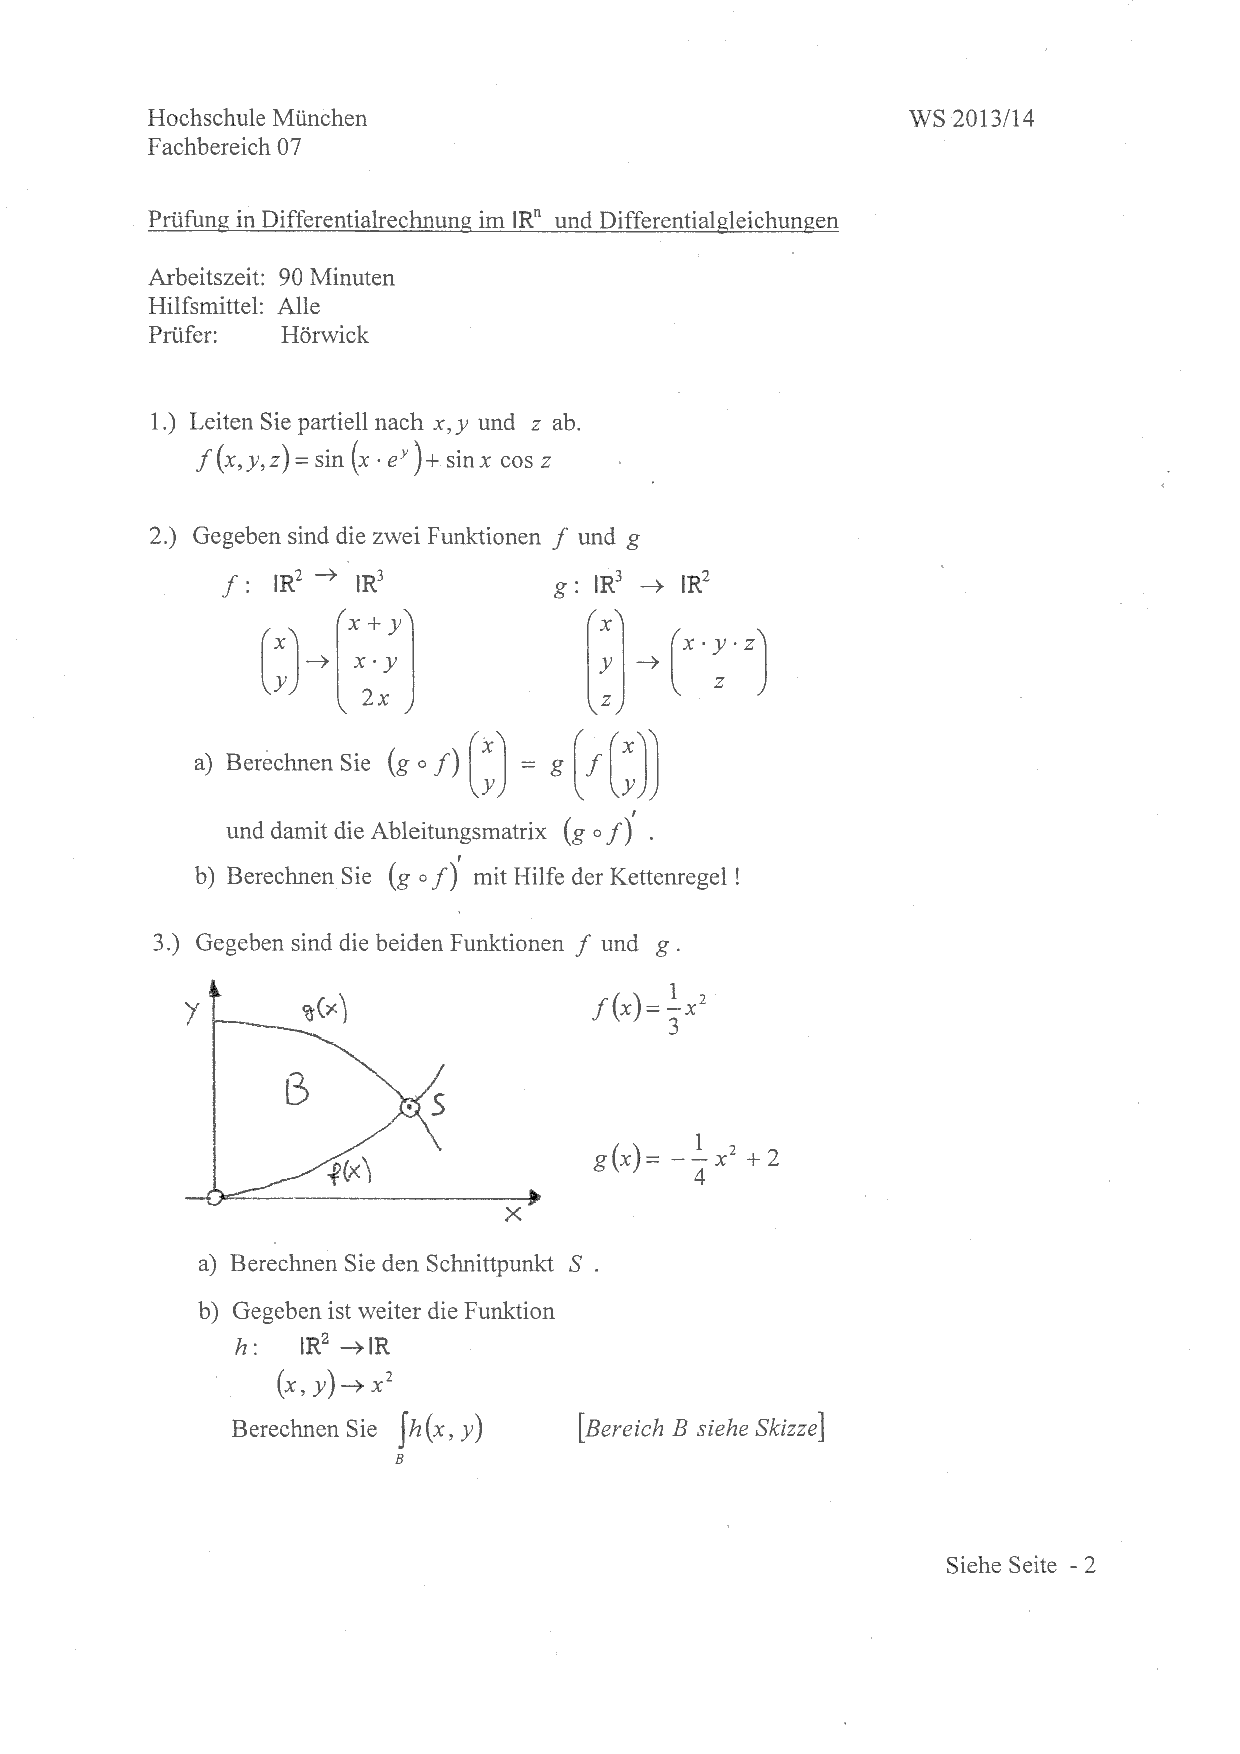
\includepdf[pages=-]{pruefungsangabe_diff_ws1314}

\section{Lösung für die Prüfung WS 2013/14}

\subsection{zu 1)}
$f(x,y,z)$
$ =\sin(x\cdot e^y) + \sin x \cos z$

$ \frac{\df}{\dx} = \cos (x\cdot e^y) e^y + \cos x \cos z$

$ \frac{\df}{\dy} = \cos (x\cdot e^y) x e^y $

$ \frac{\df}{\dz} = -\sin x \sin z$

\subsection{zu 2a)}
$ (g\circ f) \vektor{x\\y} $
$= g\vektor{x+y\\x\cdot y\\2x}$
$=\vektor{(x+y) x y 2 x \\ 2x}$
$=\vektor{2x^3y + 2x^2y^2\\2x}$

\textbf{Ableitungsmatrix:}
$ (g\circ f)' \vektor{x\\y} $
$=\vektor{6yx^2 + 4xy^2, 2x^3 + 4x^2y\\2, 0}$

\subsection{zu 2b)}
$f'\vektor{x\\y}$
$=\vektor{1,1\\y,x\\2,0}$

$g'\vektor{x\\y\\z}$
$=\vektor{yz, xz, xy\\0,0,1}$

$
(g\circ f)' \vektor{x\\y} 
=g' \rbr{f \vektor{x\\y}}  \cdot f'\vektor{x\\y}
=g'\vektor{x+y\\x\cdot y\\2x}  \cdot \vektor{1,1\\y,x\\2,0} 
=\vektor{2x^2y, 2x^2+2xy,x^2y+y^2x\\0,0,1} \cdot \vektor{1,1\\y,x\\2,0} 
=...=\vektor{6yx^2 + 4xy^2, 2x^3+4x^2y\\2,0}
$\profnote{Matrizenmultiplikation: Zeile mal Spalte!}

\subsection{zu 3a)}
$f(x) = g(x)$

$\frac{1}{3} x^2 = -\frac{1}{4} x^2 + 2$

$x=1.85 \Rightarrow y = f(1.85) = 1.14 \Rightarrow S(1.85, 1.14)$

\subsection{zu 3b)}
$
\int_{B} h(x,y) 
=\int_{0}^{1.85} \rbr{\int_{f(x)}^{g(x)} h(x,y) dy} dx
=\int_{0}^{1.85} \rbr{ \int_{\frac{1}{3} x^2}^{-\frac{1}{4} x^2 + 2} x^2 dy} dx
=\int_{0}^{1.85} \sbr{yx^2}_{y=\frac{1}{3} x^2}^{y=-\frac{1}{4} x^2 + 2} dx
=\int_{0}^{1.85} \rbr{\rbr{-\frac{1}{4} x^2 + 2} x^2 - \frac{1}{3} x^2 x^2} dx
=\int_{0}^{1.85} -\frac{1}{4} x^4 + 2x^2 - \frac{1}{3} x^4 dx
=\int_{0}^{1.85} -\frac{7}{12} x^4 + 2x^2 dx
=\sbr{-\frac{7}{12} \cdot \frac{1}{5} x^5 + 2\cdot \frac{1}{3} x^3}_0^{1.85} 
=-\frac{7}{60} \cdot 1.85^5 + \frac{2}{3} \cdot 1.85^3
=1.69
$

% Vorlesung vom 18.12.2015
\renewcommand{\ldate}{2015-12-18}

\subsection{zu 4a)}
\underline{$\varphi(0) = 1$}

$\varphi'(x) = x^2+(x-1)\cdot \varphi(x)$

\underline{$\varphi'(0) = -1$}

$\varphi''(x) = 2x + 1\cdot \varphi(x) + (x-1)\cdot \varphi'(x)$ \profnote{Produktregel!}

$\varphi''(0) = 1 + (-1) \cdot (-1) = 2$

$\varphi'''(x) = 2+\varphi'(x) + \varphi'(x) + (x-1)\cdot \varphi''(x)$

$\varphi'''(0) = 2-1-1+(-1)\cdot 2 = -2	 $

\subsection{zu 4b)}
$\varphi(h) \approx \varphi(0) + \varphi'(0) \cdot h + \frac{\varphi''(0)}{2!} \cdot h^2 + \frac{\varphi'''(0)}{3!} \cdot h^3$

$\varphi(h) \approx 1 + (-1)\cdot h + \frac{2}{2} \cdot h^2 + \frac{-2}{6} \cdot h^3$

$\varphi(0.1) \approx 1 - 0.1 + 0.1^2 - \frac{1}{3} \cdot 0.1^3 $

$\varphi(0.1) \approx 0.9097$

\subsection{EXTRA zu 4)}
Löse $y' = \underbrace{(x-1)}_{a} \cdot y + \underbrace{x^2}_{b}, \varphi(0) = 1$. Ist vom Typ lineare DGL. 

\textbf{Lösungsweg:} \profnote{Aus dem Skript}
\begin{enumerate}
\item $\varphi(x) = exp\rbr{\int_{x_0}^{x} a(t) dt}$
\item $\psi(x) = \varphi(x) \cdot \sbr{c + \int_{x_0}^{x} \frac{b(t)}{\varphi(t)} dt}$
\end{enumerate}

\textbf{Lösung}

$
\varphi(x) = exp\rbr{\int_{0}^{x} t-1 dt}
=exp\rbr{\sbr{\frac{1}{2} t^2 - t }_0^x}
=exp\rbr{\frac{1}{2} x^2 - x}
$

$ \psi(x) = exp(\frac{1}{2} x^2 - x) \cdot \sbr{1 + \underbrace{\int_{0}^{x} \frac{t^2}{exp(\rbr{\frac{1}{2} t^2 - t})}}_{f(t)} dt} $. 
$\varphi(x)$ ist die Lösung. Näherung für das Integral von 0 bis 0.1: 

$
f(0)=0, f(0.1) = \frac{0.1^2}{exp\rbr{\frac{1}{2} \cdot 0.1^2 - 0.1}} = 0.011
\Rightarrow \int_{0}^{0.1} ... dt = 0.1 \cdot \frac{1}{2} (0+0.011) = 0.00055
\Rightarrow \psi(0.1) = exp\rbr{\frac{1}{2} \cdot 0.1^2 - 0.1} \sbr{1+0.00055} = 0.90987
$

\subsection{zu 5)}
Substituiere: $z = \frac{y}{x} \Rightarrow y=xz, y'=1\cdot z + x\cdot z'$

$\Rightarrow z+x\cdot z' = \sin z + z \Leftrightarrow z' = \underbrace{\frac{1}{x}}_{f(x)} \cdot \underbrace{\sin z}_{g(z)}$ (Typ getrennte Variable). 

$\psi(1) = \frac{\varphi(1)}{1} = \frac{1}{1} = 1$

$\int_{y_0}^{\psi(x)} \frac{1}{g(t)} dt = \int_{x_0}^{x} f(t) dt$

Einsetzen der Funktionen: $ \int_{1}^{\psi(x)} \frac{1}{\sin t} dt = \int_{1}^{x} \frac{1}{t} dt $

$\sbr{\ln \tan \frac{t}{2}}_1^{\psi(x)} = \sbr{\ln t}_1^x$

$\ln \tan \frac{\psi(x)}{2} - \ln \tan \frac{1}{2} = \ln x - \ln 1$

$\ln \tan \frac{\psi(x)}{2} - \ln x = \ln \tan \frac{1}{2}$

$\ln \tan \frac{\psi(x)}{2} - \ln x = \ln 0.546$

$\ln \frac{\tan \frac{\psi(x)}{2}}{x} = \ln 0.546$ \profnote{beide Seiten e}

$\tan \frac{\psi(x)}{2} = 0.546 x$

$ \frac{\psi(x)}{2} = \arctan 0.546 x$

$\psi(x) = 2 \arctan 0.546 x$\\

$\varphi(x) = x\cdot \psi(x) = 2x\cdot \arctan 0.546 x$

\subsection{zu 6)}
$e^{i2\varphi} = $
\underline{$ \cos^2 \varphi + i \sin^2 \varphi $}

$
e^{i\varphi} \cdot e^{i\varphi} 
= (\cos \varphi + i \sin \varphi)(\cos \varphi + i \sin \varphi)
= \cos^2 \varphi + i \cos \varphi \sin  \varphi + i \sin \cos \varphi - \sin^2 \varphi
= $
\underline{$(\cos^2 \varphi - \sin^2 \varphi) + i(2\cos \varphi \sin \varphi)$}

$\Rightarrow$
\begin{enumerate}
\item $ \cos^2 \varphi = \cos^2 \varphi - \sin^2 \varphi$
\item $ \sin^2 \varphi = 2 \cos \varphi \sin \varphi \checkmark$
\end{enumerate}
 % 
% Vorlesung vom 07.01.2016
\renewcommand{\ldate}{2016-01-07}
%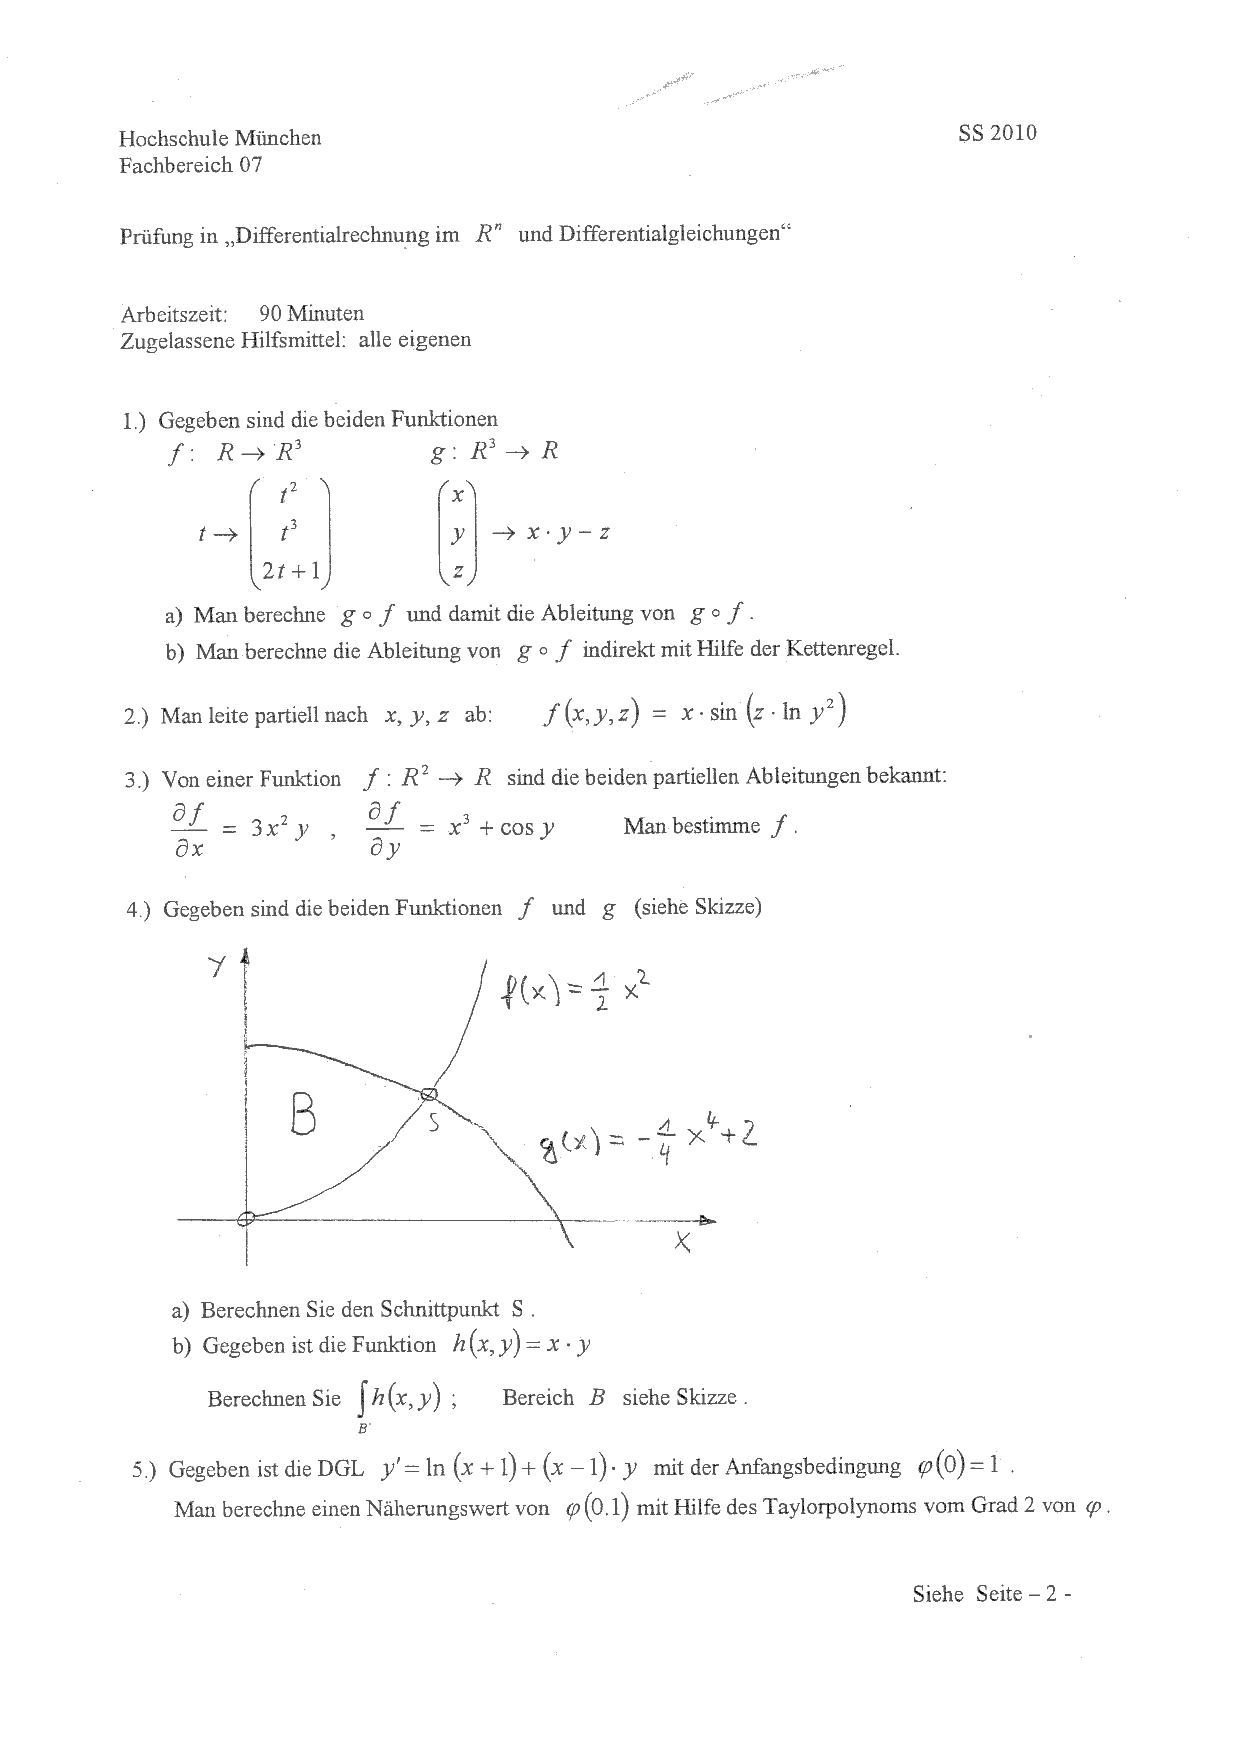
\includepdf[pages=-]{pruefungsangabe_diff_ss2010}

\section{Lösung für die Prüfung SS 2010}

\subsection{zu 1a)}
$ g\circ f) (t) = g\vektor{t^2\\t^2\\2t+1} = t^2 t^3 - (2t+1) = t^5 - 2t - 1$

$ (g\circ f)' (t) = 5 t^4 - 2$

\subsection{zu 1b)}
$ f'(t) = \vektor{2t\\3 t^2\\2}, g'\vektor{x\\y\\z} = \rbr{\frac{\delta g}{\dx},\frac{\delta g}{\dy},\frac{\delta g}{\dz}} = \rbr{y,x,-1} $

$g'(f(t)) \cdot f'(t) = g' \vektor{t^2\\t^3\\2t+1} \cdot \vektor{2t\\3t^2\\2} = \rbr{t^3, t^2, -1} \cdot \vektor{2t\\3t^2\\2} = 2t^4 \cdot 3t^4 - 2 = 5t^4 - 2 \checkmark$

\subsection{zu 2)}
$ f(x,y,z) = x\cdot \sin (z\cdot \ln y^2) = x \cdot \sin (2z \ln y)$

$ \frac{\df}{\dx} = \sin(z\cdot 2 \ln y)$

$\frac{\df}{\dy} = x\cdot \cos (z\cdot 2 \ln y) \cdot 2z \cdot \frac{1}{y} $

$\frac{\df}{\dz} = x\cdot \cos (z\cdot 2 \ln y) \cdot 2 \ln y$

\subsection{zu 3)}
Zum ersten Ausdruck: 
$ f(x,y) = 3y \cdot \frac{1}{3} x^3 + h(y) = yx^3 + h(y) $

Zum zweiten Ausdruck: 
$ f(x,y) = x^3 y + \sin y + g(x) $

$\Rightarrow h(y) = \sin y + g(x)$ In g(x) darf kein x vorkommen, also muss es eine Konstante sein: 
$ h(y) = \sin y + c$

$ f(x,y) = x^3y + \sin y + c $

\subsection{zu 4a)}
$ f(x) = g(x) $\\
$ \frac{1}{2} x^2 = -\frac{1}{4} x^4 + 2$ mit $x^2 = z$\\
$ \frac{1}{2} z = -\frac{1}{4} z^2 + 2 $\\
$ \Rightarrow z_1 = 2, z_2 = -4$\\
$z_2$ ist nicht möglich. $\Rightarrow z=2, x^2 = 2, x=\pm \sqrt{2} \Rightarrow x=\sqrt{2}$

\subsection{zu 4b)}
$ h(x,y) = x\cdot y$

$ \int_{B} h(x,y) 
= \int_{0}^{\sqrt{2}} \rbr{\int_{f(x)}^{g(x)} x \cdot y} dx 
= \int_{0}^{\sqrt{2}} \rbr{\sbr{\frac{1}{2} xy^2}_{y=f(x)}^{y=g(x)}} dx 
= \int_{0}^{\sqrt{2}} \frac{1}{2} x \sbr{\rbr{-\frac{1}{4} x^4 + 2}^2 - \rbr{\frac{1}{2} x^2}^2} dx 
= \int_{0}^{\sqrt{2}} \frac{1}{2} x \sbr{\frac{1}{16} x^8 + 4 - x^4 - \frac{1}{4} x^4} dx
= \frac{1}{2} \int_{0}^{\sqrt{2}} \rbr{\frac{1}{16} x^9 - \frac{5}{4} x^5 + 4x} dx
= \frac{1}{2} \sbr{\frac{1}{16} \cdot \frac{1}{10} x^{10} - \frac{5}{4} \cdot \frac{1}{6} x^6 + 4 \cdot \frac{1}{2} x^2}_0^{\sqrt{2}}
= 1.27
$

\subsection{zu 5)}
$ y' = \ln (x+1) + (x-1)\cdot y$ mit $ \varphi(0) = 1 $

Taylorpolynom: $\varphi(x) \approx \varphi(0) + \varphi'(0) \cdot x + \frac{\varphi''(0)}{2!} \cdot x^2$

$\varphi(0) = 1$

$\varphi'(0) = \ln(0+1) + (0-1) \cdot \varphi(0) = \ln 1 - 1 = -1$

$\varphi'(x) = \ln(x+1) + (x-1) \cdot \varphi(x)$

$\varphi''(x) = \frac{1}{x+1} + 1 \cdot \varphi(x) + (x-1)\cdot \varphi'(x)$

$ \varphi''(0) = 1 + 1 \cdot 1 - 1 \cdot - 1 = 3$

$\Rightarrow \varphi(x) \approx 1 - x + \frac{3}{2} x^2 $

$ \varphi(0.1) \approx 1 - 0.1 + \frac{3}{2} \cdot 0.01 = 0.915 $

\subsection{zu 6)}
P im u, v Koordinatensystem: 

u Wert: $\rbr{\cos \psi} + 2$ \profnote{Daheim nochmal anschauen}

v Wert: $ - \sin \psi$

$\psi$ ist die Bogenlänge (Der fette Bogen beim kleinen Kreis!).

$\psi = R \cdot \varphi = 3 \varphi$

$(u,v) = (2 + \cos \psi, -\sin \psi)$

Drehung um den Winkel $\varphi$: 

Drehmatrix: $\vektor{\cos \varphi, -\sin \varphi\\\sin \varphi, \cos \varphi}$

Koordinaten von P im xy-System:
 
$ \vektor{\cos \varphi, -\sin \varphi\\\sin \varphi, \cos \varphi} \vektor{2 + \cos 3 \varphi\\-\sin 3\varphi}
= \vektor{2\cos \varphi + \cos \varphi \cos 3 \varphi + \sin \varphi \sin 3 \varphi\\2\sin \varphi + \sin \varphi \cos 3 \varphi - \cos \varphi \sin 3 \varphi}
$

 % 
% Vorlesung vom 08.01.2016
\renewcommand{\ldate}{2016-01-08}

\section{Aufgaben}

\subsection{1.}
$f: \R^2 \rightarrow \R^2, \vektor{x\\y} \rightarrow \vektor{x^2 \sin y + y\\3y\cos x + x}$

Man linearisiere f an der Stelle $\vektor{\pi\\\pi}$:

$ f\vektor{\pi\\\pi} = \vektor{\pi^2 \sin \pi + \pi\\3\pi\cos \pi + \pi} $

$ f'\vektor{x\\y} = \vektor{\frac{\df_1}{\dx} & \frac{\df_1}{\dy}\\\frac{\df_2}{\dx} & \frac{\df_2}{\dy}} 
= \vektor{2x\sin y & x^2\cos y + 1\\ - 3 y \sin x + 1 & 3 \cos x}$ (Ableitungsmatrix)

Ableitungsmatrix an der Stelle $\vektor{\pi\\\pi}$:
$ \vektor{2\pi\sin \pi & \pi^2\cos \pi + 1\\ - 3 \pi \sin \pi + 1 & 3 \cos \pi} 
= \vektor{0 & -\pi^2 + 1\\1 & -3}$

$ f\vektor{\pi + h_1\\\pi + h_2} \approx \vektor{\pi\\-2\pi} + \vektor{0 & -\pi^2 + 1\\1 & -3} \vektor{h_1\\h_2} $

\subsection{2.}
$ y' = \underbrace{2x}_{f(x)} \cdot \underbrace{(y+1)^2}_{g(y)}$ mit $\varphi(0) = 1$

\subsubsection{herkömmliches Lösungsverfahren}
$ \int_{0}^{x} 2t dt = \int_{1}^{\varphi(x)} (t+1)^{-2} dt $ \profnote{Wegen dem Typ: $\frac{1}{g(t)}$}

$ \sbr{t^2}_0^x = \sbr{-(t+1)^{-1}}_1^{\varphi(x)} $

$ x^2 = -(\varphi(x) + 1)^{-1} + (1+1)^{-1} $

$ x^2 = - \frac{1}{(\varphi(x) + 1)} + \frac{1}{2} $

$ \frac{1}{(\varphi(x) + 1)} = \frac{1}{2} - x^2 = \frac{1 - 2x^2}{2} $

$ \varphi(x) + 1 = \frac{2}{1-2x^2} $

$ \varphi(x) = \frac{2}{1-2x^2} - 1 $

\textbf{$ \varphi(0.1) = \frac{2}{1-2\cdot 0.01} - 1 = 1.0408$}

\subsubsection{Numerische Lösung}
Versuch der Annäherung durch das Taylor-Polynom. 

$ P(h) = \varphi(0) + \varphi'(0) \cdot h + \frac{\varphi''(0)}{2} \cdot h^2 $

$ \varphi(0) = 1 $

$ \varphi'(x) = 2x \cdot (\varphi(x) +1)^2 $

$ \varphi'(0) = 0 $

$ \varphi''(x) = 2 \cdot (\varphi(x) +1)^2 + 2x \cdot 2\cdot (\varphi(x) + 1) \cdot \varphi'(x) $

$ \varphi''(0) = 8 + 0 = 8$

$\Rightarrow P(0.1) = 1 + 0 + \frac{8}{2} \cdot 0.1^2 = 1.04$

\subsubsection{Runge-Kutta-Verfahren}
Versuch der Annäherung durch das Runge-Kutta-Verfahren mit der Schrittlänge 0.1. 

$ y' = 2x \cdot (y+1)^2 = f(x,y)$ mit $x_0=0, y_0=1$

$K_1 = f(x_0, y_0) $

$K_2 = f(x_0 + 0.05, y_0 + 0.05\cdot K_1) $

$K_3 = f(x_0 + 0.05, y_0 + 0.05\cdot K_2) $

$K_4 = f(x_0 + 0.1, y_0 + 0.1\cdot K_3) $

$ K_1 = f(0, 1) = 0 $

$ K_2 = f(0.05, 1) = 8 \cdot 0.05 = 0.4 $

$ K_3 = f(0.05, 1 + 0.05 \cdot 0.4) = 0.408 $

$ K_4 = f(0.1, 1 + 0.1 \cdot 0.408) = 2 \cdot 0.1 (2 + 0.0408)^2 = 0.833 $

$ y_1 = y_0 + 0.1 (\frac{K_1}{6} + \frac{K_2}{3} + \frac{K_3}{3} + \frac{K_4}{6}) $ \profnote{Klammer: gewichtetes Mittel}

$ y_1 = 1 + 0.1 (0 + \frac{0.4}{3} + \frac{0.408}{3} + \frac{0.833}{6}) = 1.040816 ... $ 

\subsection{3.}
$ f: \R^2 \rightarrow \R^2, \vektor{x\\y} \rightarrow \vektor{2xy\\y^2}$

$ g: \R^2 \rightarrow \R^3, \vektor{x\\y} \rightarrow \vektor{x+y\\x\cdot y\\x\cdot x}$

\textbf{gesucht:} $(g\circ f)', \R^2 \rightarrow \R^3$
\subsubsection{a) $g\circ f$ berechnen, dann ableiten}

\subsubsection{b) mit Kettenregel}

Hausaufgabe

% Vorlesung vom 14.01.2016
\renewcommand{\ldate}{2016-01-14}
% 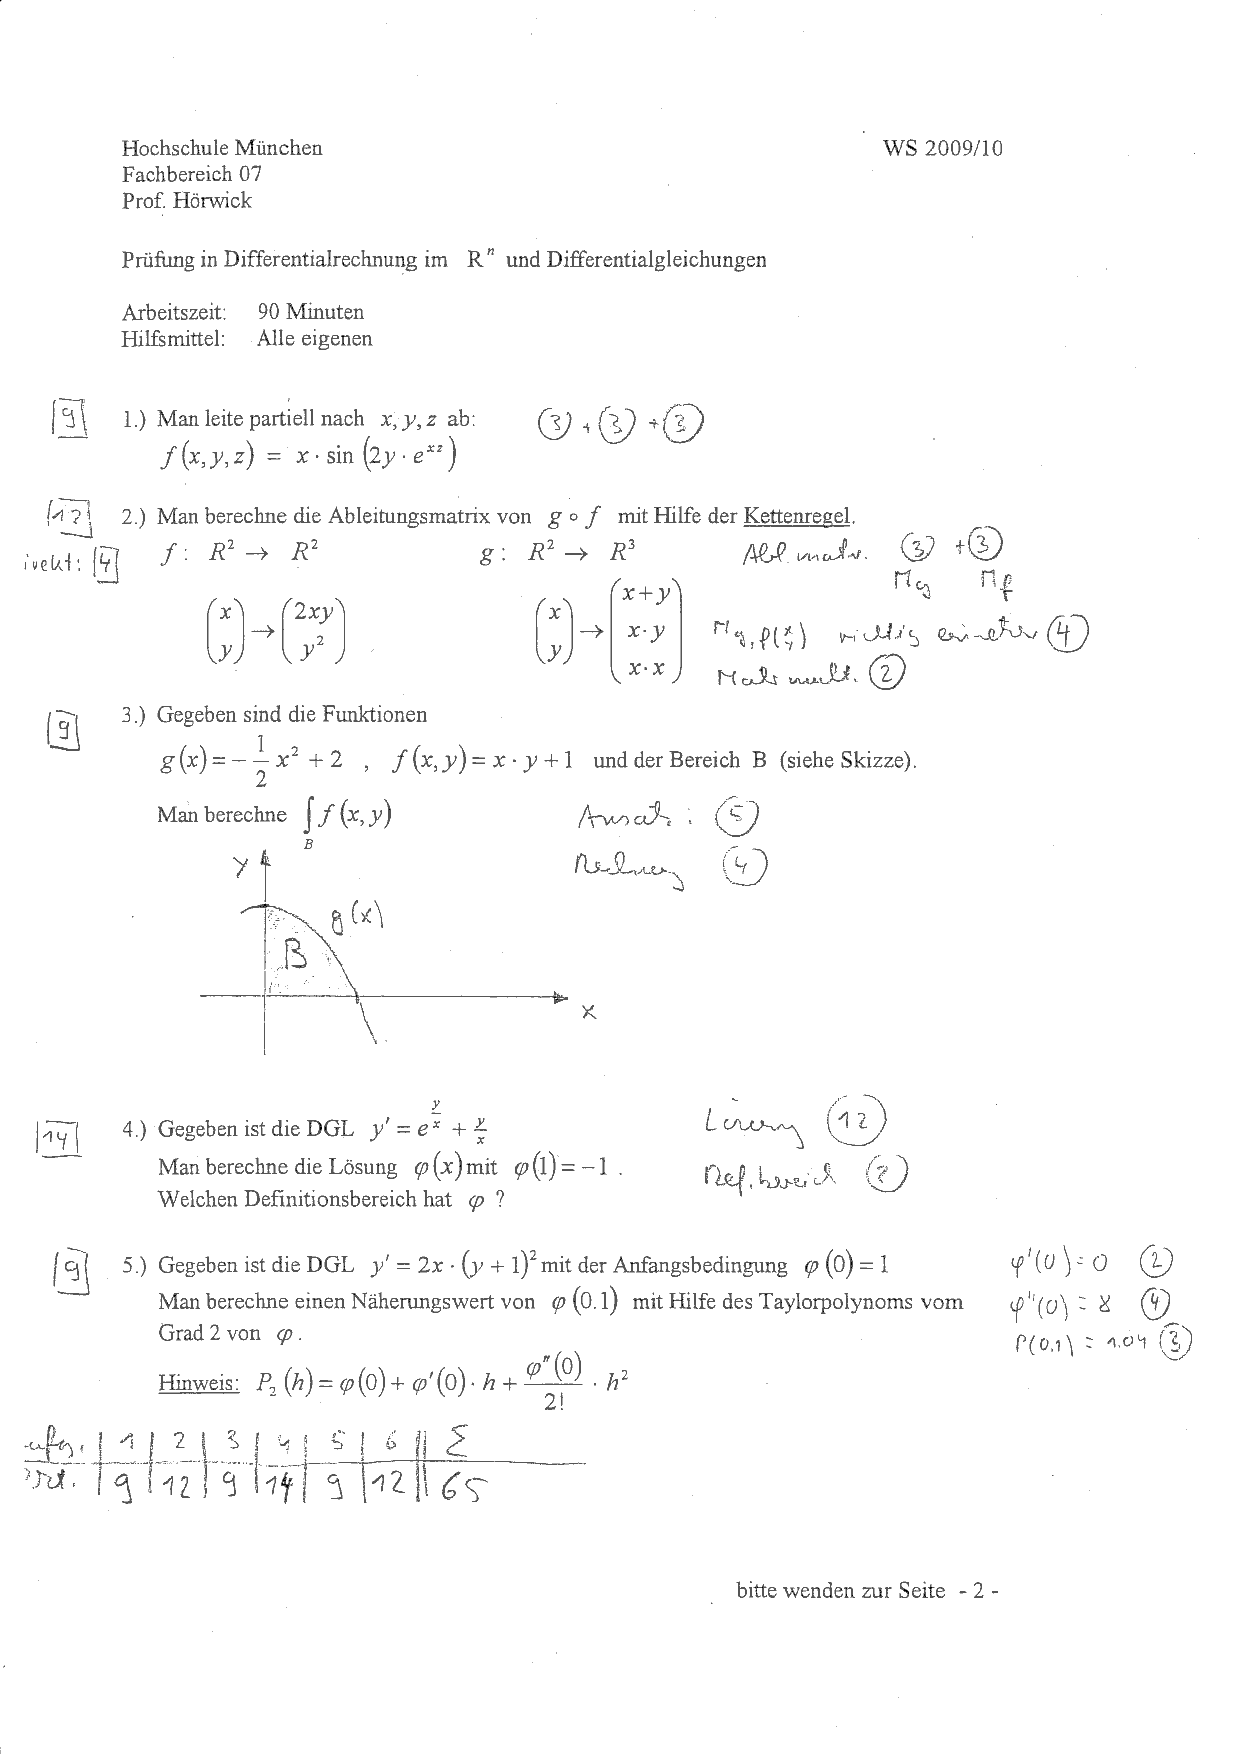
\includepdf[pages=-]{pruefungsangabe_diff_ws0910}

\section{Lösung für die Prüfung WS 2009/10}

\subsection{zu 1)}
$ f(x,y,z) = x \sin(2y e^{xz}) $ 

$ \frac{\df}{dx} = 1 \sin(2y\ e^{xz}) + x \cos(2y\ e^{xz}) 2y\ e^{xz} z $

$ \frac{\df}{dy} = x\cdot \cos(2y\ e^{xz}) \cdot 2e^{xz} $

$ \frac{\df}{dz} = x \cdot \cos(2y\ e^{xz}) \cdot 2y\ e^{xz} \cdot x $

\subsection{zu 2)}
$ f: \R^2 \rightarrow \R^2, \vektor{x\\y} \rightarrow \vektor{2xy\\y^2} $ und $ g: \R^2 \rightarrow \R^3, \vektor{x\\y} \rightarrow \vektor{x+y\\x\cdot y\\x\cdot x} $

$ (g\circ f)'(x) = g'(f(x)) \cdot f'(x) $

$ f'\vektor{x\\y} = \vektor{2y, 2x\\0, 2y} $

$ g'\vektor{x\\y} = \vektor{1, 1\\y, x\\2x, 0} $

$ (g\circ f)'\vektor{x\\y} = g' \rbr{f\vektor{x\\y}} \cdot f'\vektor{x\\y} 
= g'\vektor{2xy\\y^2} \cdot f'\vektor{x\\y}
= \vektor{1, 1\\y^2, 2xy\\4xy, 0} \cdot f'\vektor{2y, 2x\\0, 2y}
= \vektor{2y, 2x + 2y\\2y^3, 2xy^2 + 4xy^2\\8xy^2, 8x^2y, 0}
$

Kontrolle: Berechne $ g\circ f$, dann ableiten. 

\subsection{zu 3)}
\profnote{Doppelintegral. Grenze des ersten Integrals ist die Nullstelle, hier: 2.}
$
\int_{B} f
= \int_{0}^{2} \sbr{ \int_{0}^{g(x)} f(x,y) dy} dx 
= \int_{0}^{2} \sbr{ \int_{0}^{g(x)} x\cdot y + 1 dy} dx
$

$
= \int_{0}^{2} \sbr{ x\cdot \frac{1}{2} y^2 + y}_{y=0}^{g(x)=y=-\frac{1}{2} x^2 + 2} dx  
= \int_{0}^{2} \sbr{\frac{1}{2} x \cdot \rbr{-\frac{1}{2} x^2 + 2}^2 + \rbr{-\frac{1}{2} x^2 + 2} } dx
= ...
= 4
$

\subsection{zu 4)}
$ y' = \frac{y}{e^x} + \frac{y}{x} $ mit $\varphi(1) = -1$ und der Substitution 
$ z = \frac{y}{x},  y=z\cdot x, y' = z' \cdot x + z \cdot 1 \Rightarrow z' \cdot x + z = e^z + z \Leftrightarrow z' = \frac{1}{x} \cdot e^z$ (Typ: getrennte Variable)\\

Lösung $\psi, \psi(1) = \frac{-1}{1}=-1$:

$ \int_{z_0}^{\psi(x)} \frac{1}{e^t} dt = \int_{x_0}^{x} \frac{1}{t} dt$ \profnote{Jetzt brauchen wir eine Stammfunktion}

$ \sbr{- e^{-t}}_{\psi(1) = -1}^{\psi(x)} = \sbr{\ln \abs{t}}_1^x $ mit $x>0$

$ (-e^{-\psi(x)}) - (-e^1) = \ln x - \ln 1 $ \profnote{einsetzen}

$ -e^{-\psi(x)} = \ln x - e $ \profnote{Nach $\psi(x)$ auflösen}

$ e^{-\psi(x)} = e - \ln x $

$-\psi(x) = \ln (e- \ln x)$

$\psi(x) = - \ln (e- \ln x)$\\

Lösung $\varphi(x) = x\cdot \psi(x) $

$\varphi(x) = - x \ln(e - \ln x)$\\

Definition von $\varphi(x) : x > 0$

$e - \ln x > 0 $

$e > \ln x$

\underline{$ e^e > x > 0 $}

\subsection{zu 5)}
Die haben wir schon. 

%

\subsection{TEST}
\newcommand{\continue}[2]{
% defines the new command if it does not exist already
\providecommand{\num}{1}\renewcommand{\num}{1}#2#1\renewcommand{\num}{2}#2#1\renewcommand{\num}{{...}}... #1\renewcommand{\num}{{n-1}}#2#1\renewcommand{\num}{{n}}#2
}

\continue{+}{$\frac{1}{\num}$}

\continue{$\cdot$}{$t^\num$}

\continue{;}{Hallo \num}

\continue{+}{Hallo \num}

%\continue{$\varphi_{i \cdot \num} + t^{2\cdot \num+1}$}

%\continue{$2 + \num + 12$}

%$\sum_{i=1}^{n} \frac{1}{i} =$\continue{$\frac{1}{\num}$}

% Stichwortverzeichnis
% \newpage
% \renewcommand{\indexname}{Stichwortverzeichnis} % Index soll Stichwortverzeichnis heissen
% \addcontentsline{toc}{section}{Stichwortverzeichnis} % Stichwortverzeichnis soll im Inhaltsverzeichnis auftauchen
% \printindex % Stichwortverzeichnis endgueltig anzeigen
\end{document}